\documentclass{article}
\usepackage[utf8]{inputenc}
\usepackage{appendix}
\usepackage{listings}
\usepackage[svgnames]{xcolor}
\usepackage{listings}
\usepackage{graphicx}
\usepackage{tabularx}
\usepackage[hyphens]{url}
\usepackage{amssymb}

\lstset{language=R,
    basicstyle=\small\ttfamily,
    stringstyle=\color{DarkGreen},
    otherkeywords={0,1,2,3,4,5,6,7,8,9},
    breaklines=true,
    morekeywords={TRUE,FALSE},
    deletekeywords={data,frame,length,as,character},
    commentstyle=\color{DarkGreen},
}

\title{ECS 189G Term Project}
\author{Ynna Lecitona
    \texttt{yhlecitona@ucdavis.edu}
    \and Jessica Ma
    \texttt{jyma@ucdavis.edu}
    \and Duong Duy Nguyen
    \texttt{mdnnguyen@ucdavis.edu}
    \and Leo Martinez-Perez
    \texttt{leomartinezp@ucdavis.edu}
    \and Tycho Yacub
    \texttt{tsyacub@ucdavis.edu}
}
\date{Spring 2020}

\begin{document}

\maketitle

\section{Introduction}
All quarter we've been predicting item ratings in the format of, "User i rates item j as x", where x is the predicted rating. To take it one step further, the goal of this project is to report the probabilities of a user i, rating item j from min to max rating. For example, for user 20 and movie 10, the probabilities of rating it a 1, 2, 3, ... are 0.102, 0.373, 0.111, ... respectively. 

$\newline$
The main goal of the project is to calculate these probabilities through the use of 4 prediction methods: logit, NMF, kNN, and CART. Some restrictions presented include: the user being able to embed means, the user specifying any method-specific arguments like amount of trees for CART, rank for NMF, etc. After completing a working model for each prediction, we chose to compare the accuracies of the various types of prediction methods using two datasets: InstEval and Song List. 

$\newline$
The InstEval dataset includes university lecture evaluations by students at ETH Zurich. In the InstEval dataset, we chose to trim the data to only include the student, instructor, and rating as specified by our models' constraints. 
The Song List dataset includes information about how a certain user rates a specific song. 

\section{Logit}

\subsection{Introduction to the Logistic Regression Model}

In classification problems, one often wishes to predict whether or not a collection of data pertains to a specific category. In order to achieve this, we can use a logistic regression model to predict the mean of a binomially distributed indicator variable that indicates whether the data belongs to the category. This mean will be within the range [0,1] and represent the probability that the variable will be equal to 1. In our case our indicator variables will be whether or not the user gave the item the rating r, where r represents all possible ratings that could be given to the item. 

$\newline$
This method utilizes the logistic function, $\frac{1}{1+e^{-\mu}}$, where $\mu$ is a model of the different users and items multiplied by linear parameters, $\beta_0 + \beta_1x_1 + ... + \beta_nx_n$. These parameters can be estimated iteratively through the Maximum Likelihood Estimation method by being exposed to a set of training data. 

\subsection{Implementation of Logit}
Logit was implemented by using the built-in R function "glm". Glm stands for generalized linear models and supports several parametric families. In order to use logit we must specify to use the binomial family. The implementation of our code draws inspiration from the One vs. All method. The One vs. All method is used when one is attempting to categorize something that could belong to one of several categories. In order to determine a prediction for which category the data belongs to, we can create a separate model for every single category and categorize it corresponding to whichever model yields the most certain prediction. In our case, however, we are not attempting to categorize the data. Therefore we can simply generate n different models, where n is the number of possible ratings. We can then return these models inside of an R S3 object or a list.

$\newline$
This object can then generate the probabilities that the a given user would rate a given movie a certain rating by using the built-in R function 'predict'. Predict.glm takes in a general linear model, the new data to predict, and the optional parameter of type = 'response', which indicates to the function that the prediction should be a probability. In order to generate the probabilities for every possible rating, we must call predict for every single glm model that was generated from the ratingProbsFit function.

\subsection{Shortcomings of Logit}
During the exploration of the Logit method for classification, we encountered a couple of shortcomings that make it difficult to use Logit in every situation.

$\newline$
A common question asked in computer science is, "does it scale"? Unfortunately, when testing our implementation of Logit one of the first issues we noticed was that the time complexity to generate logistic regression models for every possible rating was very large. When handling data points like userID and itemID with many factors, glm must create dummy variables for every single level. As a result, it would take approximately thirty minutes to finish computing the probabilities for a data set of 10,000 rows on our personal computers. Assuming a linear increase in time as we increased the number of rows, to run glm on a dataset of a million rows it would take us 50 hours. 

$\newline$
Another issue with using Logit for classification is that it does not account for new users or items. If the training model has not been exposed to a user or an item when attempting to predict it will not know what to do. As a result, if you wished to introduce new users or items you would have to recompute the entire model. On a similar note, one must be extremely careful when partitioning the data into a training set and testing set during cross validation for Logit. This is because, one must ensure that every item and movie within the testing set is present in the training set. 

\subsection{Testing the Effectiveness of Logit}
\subsubsection{InstEval Data Set}
The first data set which we used to test Logit was the InstEval data set. The InstEval data set represents a collection of students, instructors, and ratings of the lecturers from one to five. Due to the scale of the data set, we decided to trim the data set such that only the first 10,000 rows are used. In order to partition these 10,000 rows into a training and testing set we used an algorithm found on Stack Overflow. This code could be found on Appendix E.

$\newline$
This code takes a random sample of 95\% of the total data for the training set and the remaining 5\% for the testing set. It then checks to see if the testing set is a subset of the training set. If it isn't it creates another random partition of the data and checks again until it is valid. 

$\newline$
After using this partition to determine the probabilities of each possible rating, we can save the data set to a file in order to analyze it. One of the first things we did to verify the validity of our data set was to ensure that every row added up to one and thus represented a complete view of all the possible ratings that could occur. In our case it added up to approximately one. We attributed this to rounding errors with the significant figures reported by R.

\begin{figure}[ht]
\centering
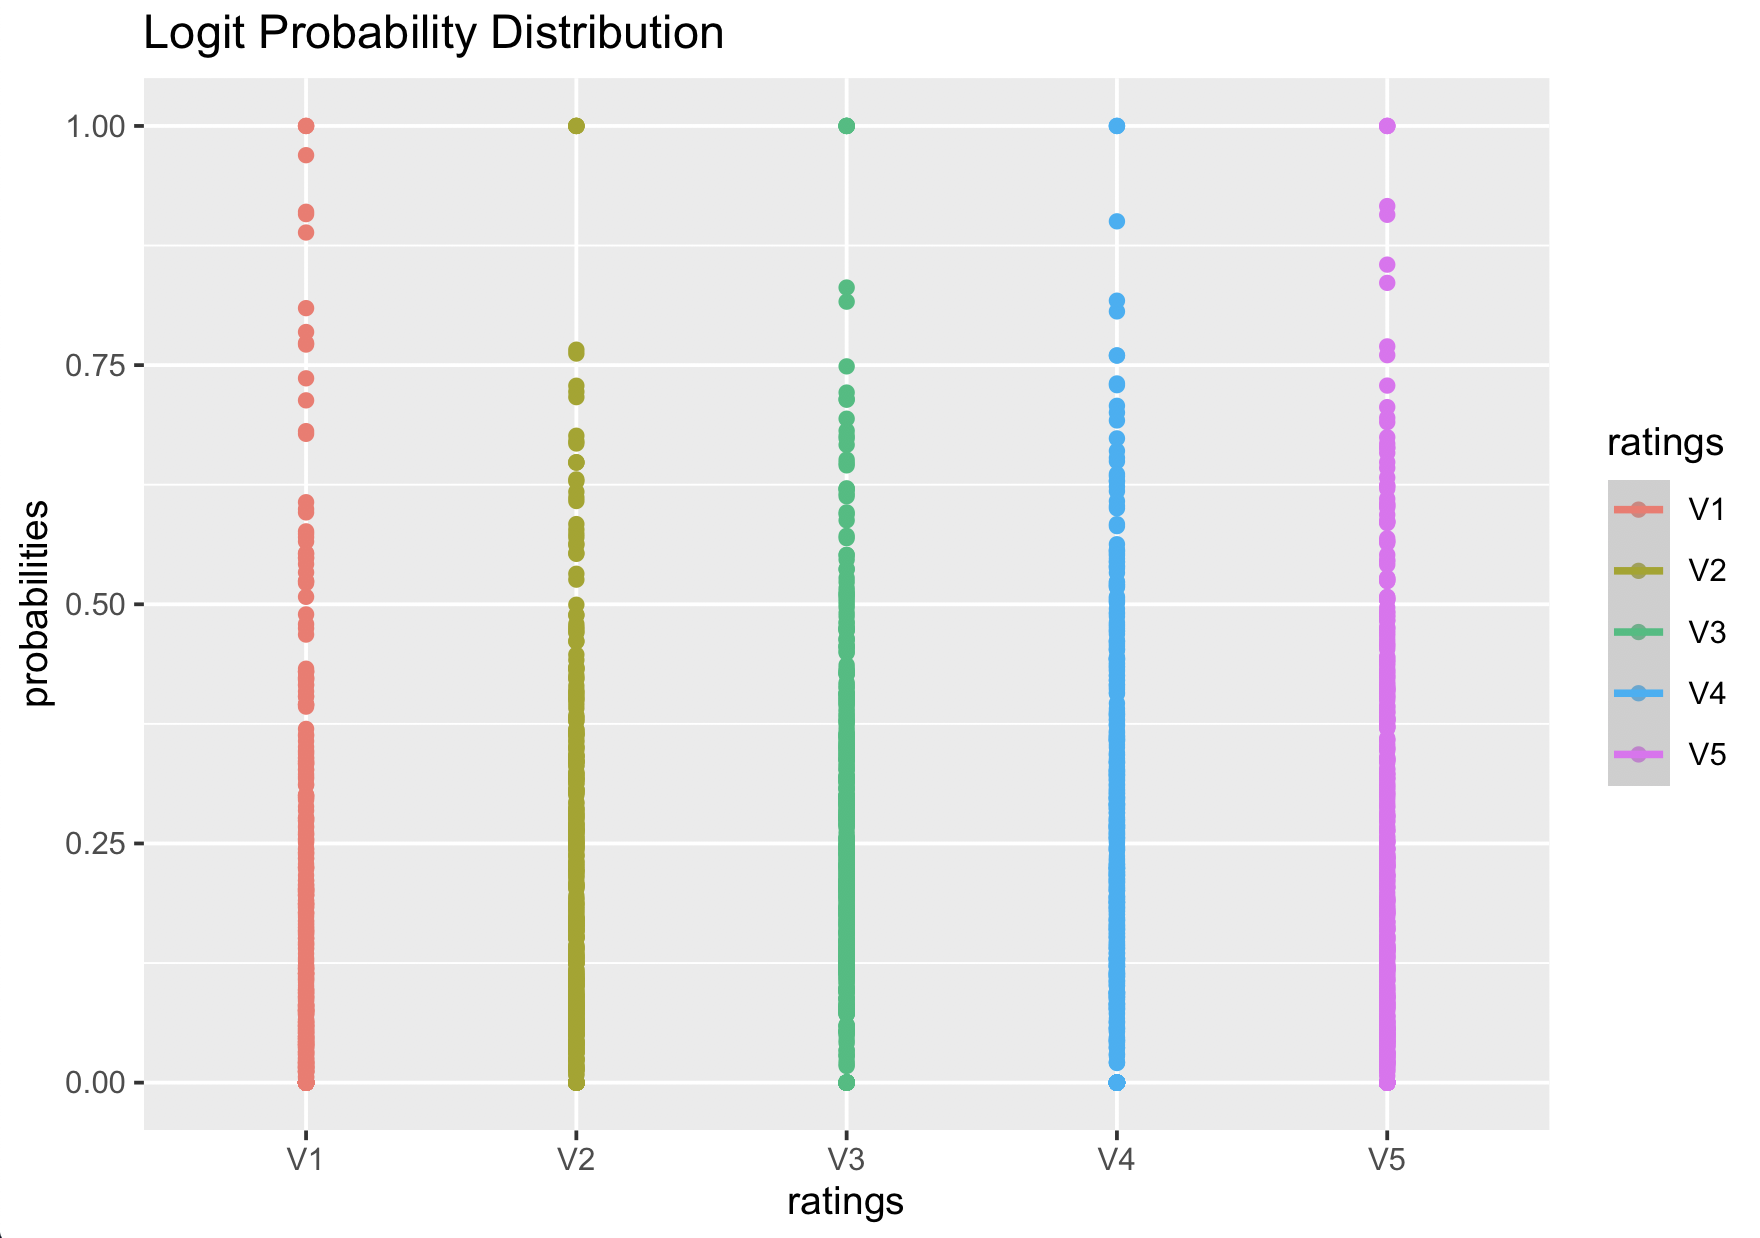
\includegraphics[scale=0.3]{Logit InstEval Prediction Probability Distribution.png}
\caption{Logit Probability Distribution}
\label{fig:universe}
\end{figure}

$\newline$
In order to analyze the probabilities outputted by Logit, we decided to plot the probabilities such that it would reflect a probability distribution of all the ratings (Figure 1: Logit Probability Distribution). From first glance, we can notice that there are some probabilities that were automatically fitted to be zero or one. This can be seen in the points which lie on the probabilities = 1 axis. We suspect that this may be because of outliers in our data. If one wanted to explore deeper into this, they could make note of the userIDs and itemIDs that are generating fitted probabilities. They could then extract the glm objects outputted by ratingProbsFit and analyze the standard error reported for those userIDs and itemIDs. 

$\newline$
We also noted that the probability distribution somewhat resembled that of a binomial distribution graph generated by a histogram. This is because there appears to be a peak at a rating of three and as the rating strays from the peak its probability is reduced on average. This is what we expected to see because we generated the linear regression such that the rating modeled a binomial distribution.

$\newline$
The raw output of the probabilities can be found in the LogitPredictions.data file submitted with this project. The LogitPredictions.data are the probabilities predicted from the TrimmedTest.data file after training our model on the TrimmedTrain.data.

\subsubsection{Song List Data Set}
The second data set which we used test Logit was the Song List data set. The Song List data set represents a collection of users, songs, and the ratings of those songs from one to five. Much like the InstEval data set we opted to only use the first 10,000 rows of the data set and we partitioned it using a 95\%/5\% split. 

However, our algorithm was unable to find a successful partition after about an hour of attempts. This prompted a deeper look at the code that we were analyzing. We noticed that there were 200,000 unique users and 127,771 unique songs within this data set. Therefore we increased our data set to be first 100,000 rows of the original data set. In this case, we were also unable to find a successful partition after attempting to do so for a long time. 

We could greatly increase our chances of finding a successful partition if we were to increase the size of the data we were using. However, the computation of the probabilities would be unfeasible to run on our personal computers. As a result we were forced to omit the analysis of the probabilities produced by Logit on the Song List data set. 


\section{NMF - Nonnegative Matrix Factorization}

\subsection{Introduction to Non-negative Matrix Factorization}

NMF is the process of decomposing a sparse matrix into two matrices that approximate the values already present in the matrix. This allows us then to approximate values in the matrix that we do not have data on. Therefore, NMF is a strong choice of model in recommender systems when all users and items are already known.

\subsection{Implementation}

The most important choice to make when using NMF is the choice of rank. This rank determines the granularity at which our synthetic users and items are generated. This means that making the right choice of rank is crucial. 

To do this when a user inputs their data into probRatingsFit() with the method 'NMF' they have the choice of choosing their own rank in the specialArgs. However, we also give the user the option of not inputing a rank and having that determined for them. In the case that they do not input a rank we use RecoSystem's tune() function to run crossvalidation across the ranks [25, 50, 100, 200] we felt that this would give the user a good overview of what range of ranks will work best for them. 

Unfortunately though you can also tune parameters like learning rate and regularization functions the number of possible combinations of rank and other hyper parameters makes optimization take days to run.

\subsection{Testing}

Running NMF began with the data from MovieLens. This data ran extremely quickly and well with the crossvalidation function that we made ourselves. Below you can see the lowest loss values for MovieLens and SongList.

\begin{figure}[ht]
\centering
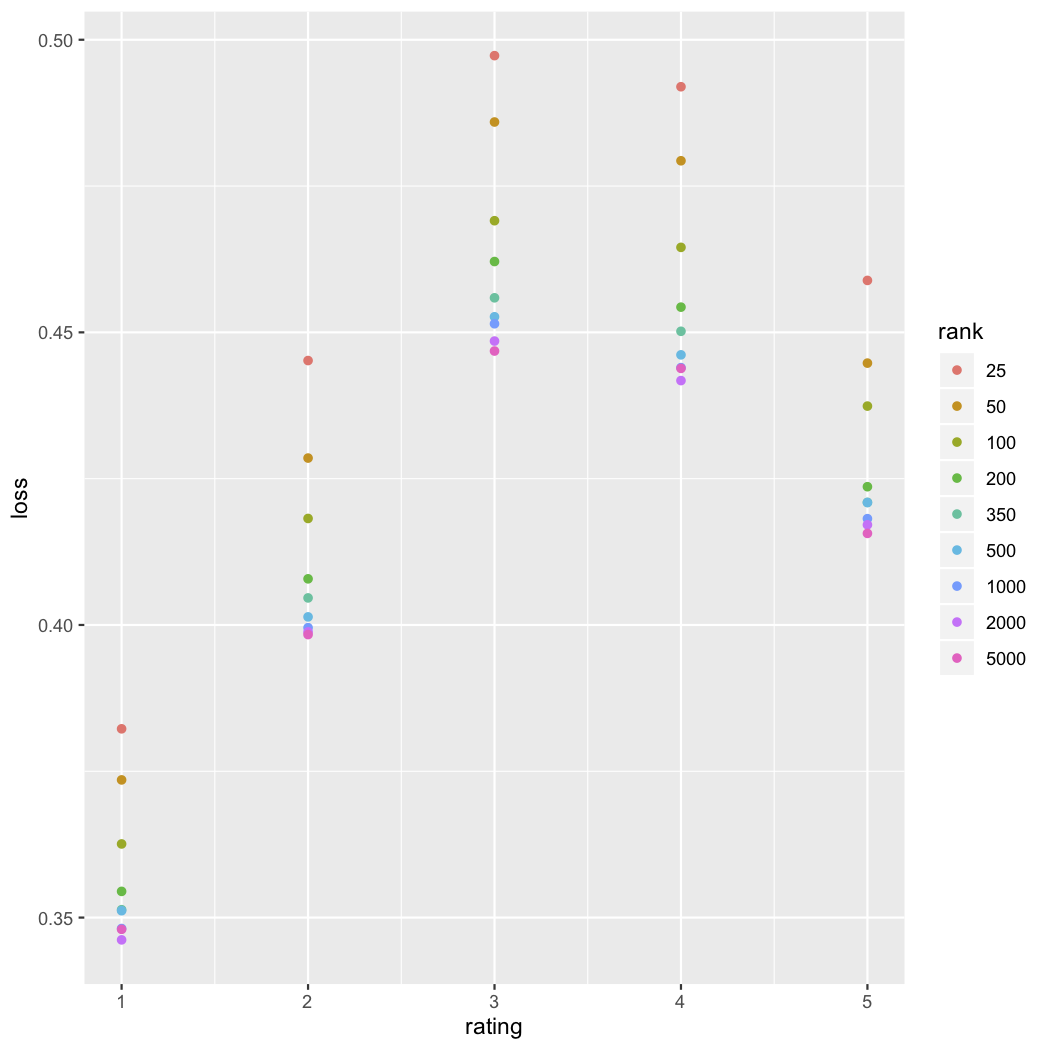
\includegraphics[scale=0.3]{FinalNMFMovie.png}
\caption{MovieLens Rank x Loss}
\label{fig:universe}
\end{figure}

\begin{figure}[ht]
\centering
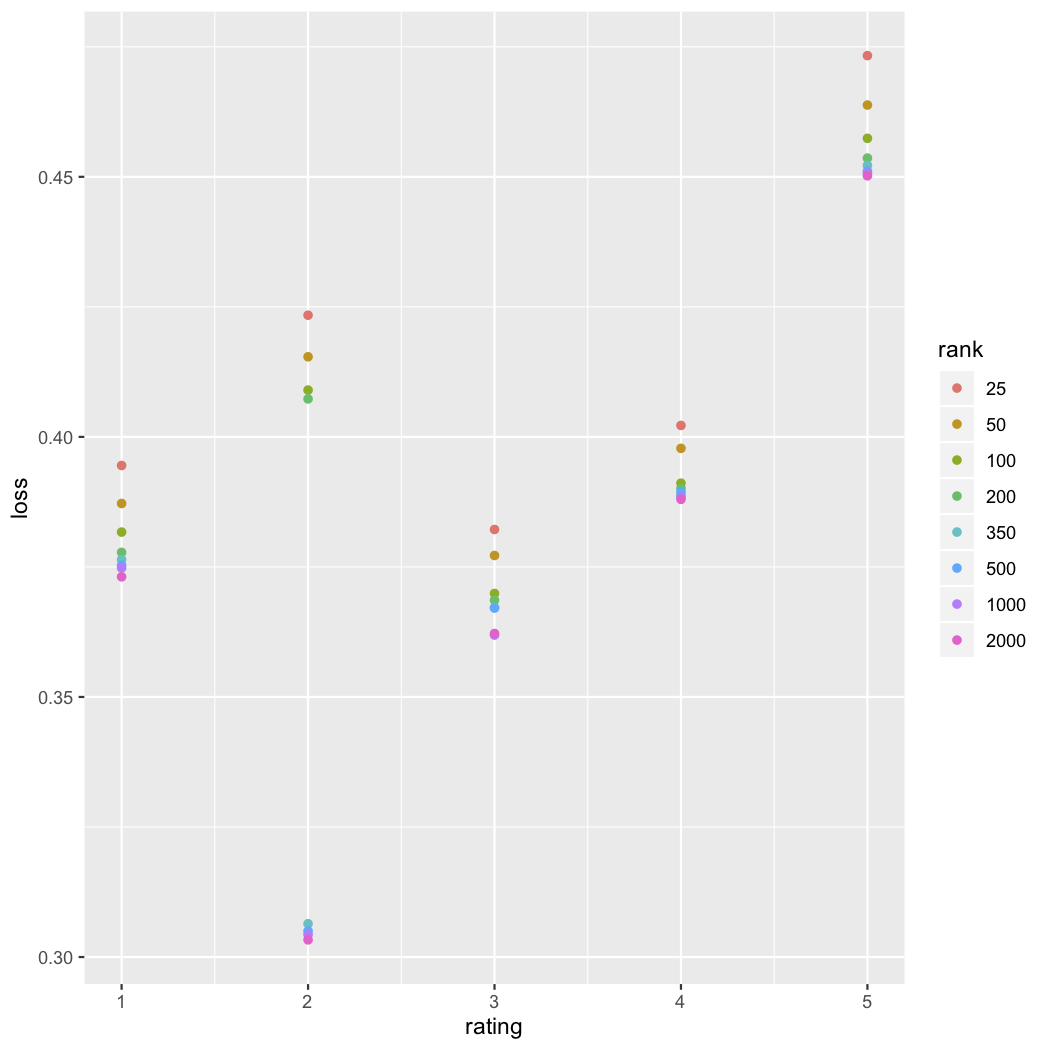
\includegraphics[scale=0.3]{FinalNMFSong.png}
\caption{SongList Rank x Loss}
\label{fig:universe}
\end{figure}

As you can see the loss value continued to drop. Unfortunately, it was not able to run long enough to get higher rank value. Though we can see that change in loss begins to get very small and that likely we were close to the optimal rank.

\section{KNN - k Nearest Neighbors}

\subsection{Overview}

The kNN algorithm can, given a data point p, determine the k other points in the dataset that are most "similar" to p. Said similarity metric can be calculated using a similarity function--any function whose output changes according to how similar in value one data point is to another.

For our project:

\begin{enumerate}
    \item The data points are rating vectors, where each vector contains a user's ratings for all available items.
    \begin{itemize}
        \item Items that a user hasn't rated will have a rating of NA.
    \end{itemize}
    \item We view the higher the similarity value between two vectors, the more similar those two vectors are.
    \begin{itemize}
        \item Similarity values can be either positive or negative.
    \end{itemize}
    \item If a user has less than k nearest neighbours, we'll use as many as there are available.
\end{enumerate}

Given a user U and an item I that said user has never rated before, by using kNN's similarity metric, we can find the k users who have rated I that are most similar to user U, and, based on their ratings of item I, predict what rating would user U most likely give for item I.

Although we found the idea behind kNN to be intuitive, implementing a general kNN program within R proved quite challenging, mainly in these areas:
\begin{enumerate}
    \item Choice of data format
    \item Choice of similarity function
\end{enumerate}

\subsection{Choice of data format}

\subsubsection{Matrix format}

Since the kNN method requires access to specific user rating vectors in its calculation, we initially decided on representing the input dataset as a matrix. Each row would represent a user, each column would represent an item, and each entry in the matrix would represent a rating. As mentioned before, items that a user hasn't rated would have a rating of NA. 

Initially, this format worked quite well, as we were able to perform prediction on the InstEval dataset, using 51394 known ratings (train set) to predict 14684 new user and item entries (validation set), in roughly 1 minute. 

\begin{figure}[ht]
\centering
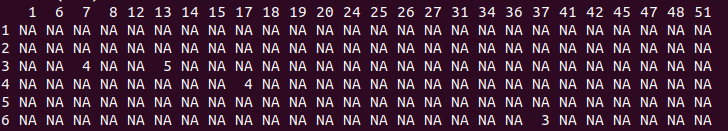
\includegraphics[scale=0.5]{Matrix.png}
\caption{Rating Matrix}
\label{fig:universe}
\end{figure}

\subsubsection{data.frame format}

However, the problem arose when we tried to run our kNN program on SongList, a medium size dataset with 2 million entries. With 200 thousand unique users and more than 127 thousand unique items, the resulting rating matrix was too large to be represented in R.

Following the recommendation in the textbook, we first tried to represent the SongList dataset using the rectools package's \textbf{formUserData()} function. However, the convertion took too long so we gave up on this idea.

Then, we tried switching to using a simple \textbf{data.frame} structure to represent the input dataset. Now, whenever kNN requires a specific user rating vector, we would search through the input dataset, find all ratings belong to the specified user, and construct said vector. This meant that for a user U and k neighbors, we would perform the searching k+1 times. With this method, we could finally handle SongList. 

However, said dataset searching and rating vector construction lead to a \underline{severe decrease in performance}. Using the same InstEval prediction case as above, this new data format finished prediction in roughly 6 minutes. Even worse, when we tried running our kNN program on Song List, using 1.6 million known ratings (train set) to predict 200 thousand new user and item entries (validation set), the program didn't finished \textbf{even after nearly 30 hours}.

\subsubsection{Hybrid format}

Knowing that the main problem lied in the searching, we decided to combine our two formats together. The overall input data set would still be a \textbf{data.frame} object, but for every prediction of a certain user U and an item I, we would

\begin{enumerate}
    \item First extract the ratings of all users who have rated item I--as well as that of user U--from the input data set (using indexing)
    \item Then, we would construct a matrix from the extracted data set.
    \item Finally, we would perform kNN using said matrix. 
\end{enumerate}

With this hybrid format, we successfully performed kNN on SongList in roughly \textbf{3 hours}, a significant decrease from 30 hours.

Moreover, we discovered that with this format, for any one prediction instance, the matrix that we had to use was \underline{much smaller than the one created by} \underline{converting the entire input data set}.

This effect stemmed from two reasons:

\begin{enumerate}
    \item At any instance, we only considered (and then converted to matrix) a small portion of the users in the data set. Therefore, the resulting matrix had \textbf{much less rows}.
    \item At any instance, regarding the users we considered, the combine total number of unique items that they have rated was only a portion of the number of unique items in the data set. Therefore, the resulting matrix had \textbf{much less columns}.
\end{enumerate}

We regarded this space-saving result to be a good tradeoff for the matrix construction we had to perform for every new prediction request.

\subsubsection{Matrix format + hybrid format}

However, for smaller data sets like InstEval, this method wasn't ideal, as we could have used the matrix resulting from the first format in all of our predictions--thereby going from O(n) to O(1) regarding data set setup. 

Therefore, we decided to combine the techniques again, this time regarding data set size. For data sets that can be entirely presented with an R matrix, we would use the first format; for data sets that couldn't, we would use the hybrid format. This ensured the best of both worlds in terms of both time and space complexities.

\subsection{Choice of similarity function}

Considering that kNN revolves around the idea of similarity, we believe that choosing a good similarity function is very important. Therefore, we searched the Internet for potential similarity functions and found 8 different ones. Moreover, based on our observations of the found similarity functions' behaviors, we also made 1 of our own.

\subsubsection{Cosine similarity}

This is one of the most common ones because of its intuitive idea, simple calculation, decent results.

\subsubsection{Manhattan, Euclidean, and Chebychev similarities}

These are l-p norm functions with different values for p (1 for Manhattan, 2 for Euclidean, and infinity for Chebychev), depicting the distance between two points. We calculated similarities by dividing these distances from 1. Therefore, the less total distance between two vectors' elements, the higher the similarity score. 

While they have similar advantages as the cosine similarity function, the results they produced for InstEval were slightly worse (except for Chebychev, which sometimes produced slightly better results than Cosine).

\subsubsection{Jaccard similarity (not considered)}

Unlike the previous 4 which involves more geometry, Jaccard similarity comes from set theory and has a simple idea: the more elements 2 sets share, the more similar they are to each other. 

This is acceptable in the set case, but doesn't translate well in our (user,item) scenario. Just because two users have rated the same item doesn't mean they are more similar to each other--their ratings of said item also matter. Therefore, \underline{we didn't keep this function in our program}.

\subsubsection{Dot product similarity (not considered)}

This function is the numerator of the fraction that computes the Cosine similarity. While the Google Developers website suggested this as a possible similarity function, we found a major flaw in its working--this method relies too much on the actual value of a variable, instead of how similar said value is to the corresponding one of another variable. 

For example:

Vectors (0,3) and (0,3) has a dot product value of 9

Vectors (0,3) and (0,5) has a dot product value of 15

Vectors (0,3) and (0,1) has a dot product value of 3

We can see that there isn't a clear way to tell which pair is more similar based only on the value, even though it should be obvious that the answer is the first pair. Therefore, \underline{we didn't keep this function in our program}.

\subsubsection{Correlation similarity}

We came up with the idea of using correlation as a similarity metric for our kNN, then found a website that supported it (see Section H). The gist is that if two users are similar to each other in terms of rating behavior, when one user rates an item highly, the other user should also rate similarly. This is a behavior that correlation represents. 

In terms of results, this function performs surprisingly well, \underline{being even better} \underline{than the Cosine similarity}.

\subsubsection{Radial basis function kernel similarity}

While this kernel function sees more use in support vector machine classification, according to Wikipedia, its value "decreases with distance and ranges between zero...and one...(and therefore has) a ready interpretation as a similarity measure." 

Testing shows that its performance was slightly worse than Cosine similarity.

\subsubsection{Inhouse function}

Our similarity function was motivated by the following observations of the Cosine similarity function:

Given 3 vectors a, b, and c. If the angle between a and b is different from the angle between a and c, then the Cosine similarity can determine which of b and c are more similar to a. However, said prediction based on the angle between 2 vectors \underline{isn't always right}.

\begin{enumerate}
    \item If the angle between a and b is the same as that between a and c, Cosine similarity would view b and c as equally similar to a, regardless of the vectors' length.
    \begin{itemize}
        \item Ex: a = (1,2), b = (1,2), c = (2, 4).
        \item The angle between a and b and that between a and c are both 0 => cos(0) = 1 for both cases. However, we can see that b is more similar to a and c is--in fact, b is exactly a. But the cosine similarity can't capture that.
    \end{itemize}
    
    \item Moreover, even if the angle between a and b is smaller than that between a and c, that doesn't necessary mean that b is more similar to a than c.
    \begin{itemize}
        \item Ex: a = (1,2), b = (2,4), c = (1, 3).
        \item The angle between a and b is 0, while that between a and c is slightly higher than 0. However, we argue that c should be more similar to a than b. This isn't the case, however, with Cosine similarity.
    \end{itemize}
    
    \item Finally, if the angle between a and b is equal to that between a and c, but b has more similar elements than c, b should be more similar. Once again, the Cosine similarity function doesn't capture that.
    \begin{itemize}
        \item Ex: a = (1,2,3), b = (1,2), c = (1,2,3).
        \item The angle between a and b and that between a and c are both equal to 0 in their respective dimension. However, we argue that c is more similar because of the extra value in the 3 element.
    \end{itemize}
\end{enumerate}

To handle these 3 problems, we came up with the following function: Given a potential user rating vector V1 and our target user rating vector V2 (the vector for user U):

\begin{enumerate}
    \item Find the length of the projection of V1 on V2: P1 = $V1 * V2 / \vert \vert V2 \vert \vert$
    
    \item Find the length of the projection of V3--the difference of V1 and V2--on V2: $P2 = V3 * V2 / \vert \vert V2 \vert \vert$
    
    \item Calculate the difference: $D = P1 - P2$
    
    \item Multiply the result by the Cosine similarity: $D * cosineSim(V1, V2)$
\end{enumerate}

\begin{figure}[ht]
\centering
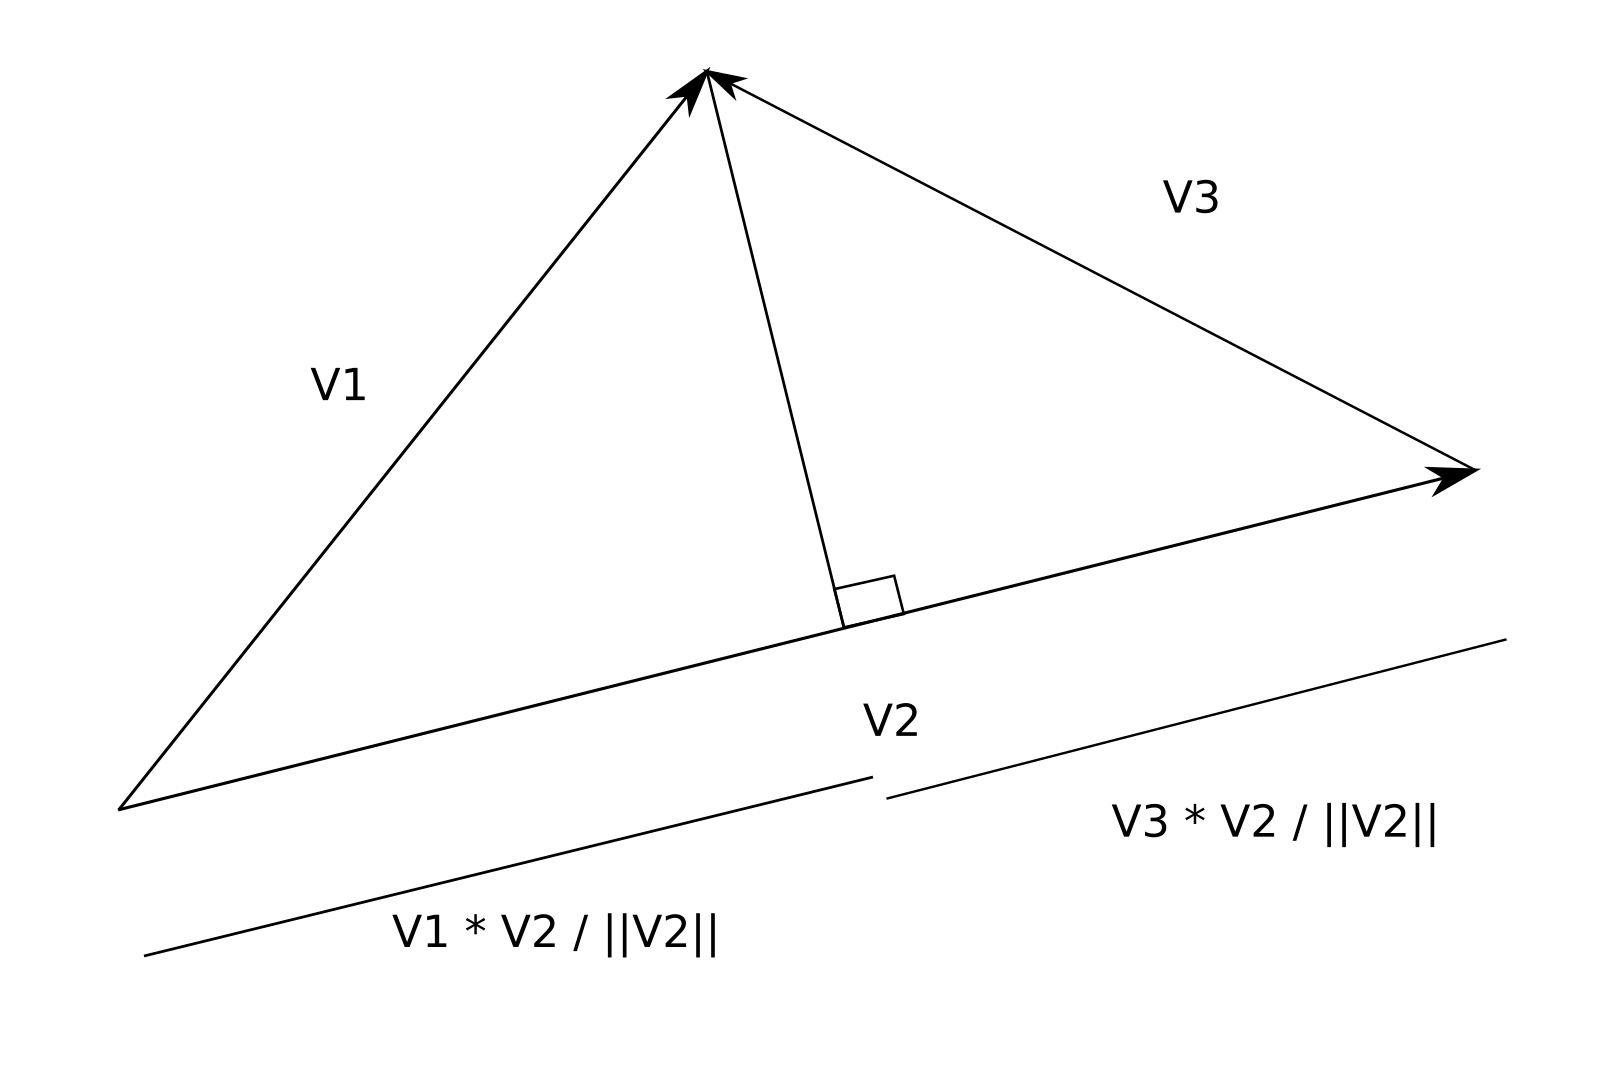
\includegraphics[scale=0.2]{inhouse.png}
\caption{Inhouse function}
\label{fig:universe}
\end{figure}

Our reasoning is that the difference between the projection lengths can help us solve the problems stated in the observations above. 

However, we eventually found out that said approach only helped with problem c and not problem a or b. 

\begin{itemize}
    \item It turns out that increasing the size of V1 by a certain factor results in V3 decreasing by the same factor and vice versa. Therefore, difference between the projection lengths stays the same and problem a wasn't solve.
    
    \item Since problem a wasn't solve, the similarity between (1,2) and (2,4) is the same as that between (1,2) and (1,2). Therefore, problem b wasn't solved as well.
    
    \item However, because we took vector lengths into consideration, the more elements V1 and V2 shares, the larger the projection length value. Therefore, problem c was solved.
\end{itemize}

Even though we only solved 1 out of 3 problems that we observed with the Cosine similarity, said solution increased our prediction accuracy by a few percents. Moreover, because we have the cosine value multiple, we also got the benefits of Cosine similarity in our function. Therefore, we decided was enough to choose our inhouse function as the main similarity function for this project.

\subsection{Results}

To measure accuracy, we took the rating probability matrix from kNN and find the rating with the highest probability for each entry. We then compare those ratings to the ones from our validation sets and calculated the percentage of ratings we got right. 

Following is the result for each similarity function discussed above (except for Jaccard similarity and Dot Product similarity). 

The testing scenario is the InstEval dataset, with 51394 entries in the input data set, 14684 entries in the validation set, and 7343 entries in the test set. 

For k equals 5:

\begin{center}
    \begin{tabular}{c|c|c}
        Similarity Function & Validation Data & Test Data \\
        \hline
        Cosine & 0.3396895 & 0.3309274 \\
        Manhattan & 0.3356034 & 0.3343320 \\
        Euclidean & 0.3378507 & 0.3348768 \\
        Chebychev & 0.3377826 & 0.3408689 \\
        Correlation & 0.3452057	& 0.3479504 \\
        RBFK & 0.3378507 & 0.3348768 \\
        Inhouse & 0.3554209 & 0.3587090 \\
    \end{tabular}
\end{center}

For k equals 10:

\begin{center}
    \begin{tabular}{c|c|c}
        Similarity Function & Validation Data & Test Data \\
        \hline
        Cosine & 0.3332198 & 0.3250715 \\
        Manhattan & 0.3329474 & 0.3249353 \\
        Euclidean & 0.3325388 & 0.3297018 \\
        Chebychev & 0.3344457 & 0.3333787 \\
        Correlation & 0.3390765 & 0.3369195 \\
        RBFK & 0.3325388 & 0.3297018 \\
        Inhouse & 0.3495642 & 0.3384175 \\
    \end{tabular}
\end{center}

We can see that our similarity function produced better results, even if only slightly, than other similarity functions. This justifies our decision to use our inhouse function as the main similarity function for this project. 

Running our kNN program on the SongList dataset, with 1600000 entries in the input data set, 200000 entries in the validation set, and 200000 entries in the test set, we get the following results:

\begin{center}
    \begin{tabular}{c|c|c}
        k & Validation Data & Test Data \\
        \hline
        5 & 0.41884 & 0.414995 \\
        10 & 0.42199 & 0.41969 \\
    \end{tabular}
\end{center}

\subsection{Distributions and Graphs}

\subsubsection{For InstEval}

\begin{figure}[ht]
\centering
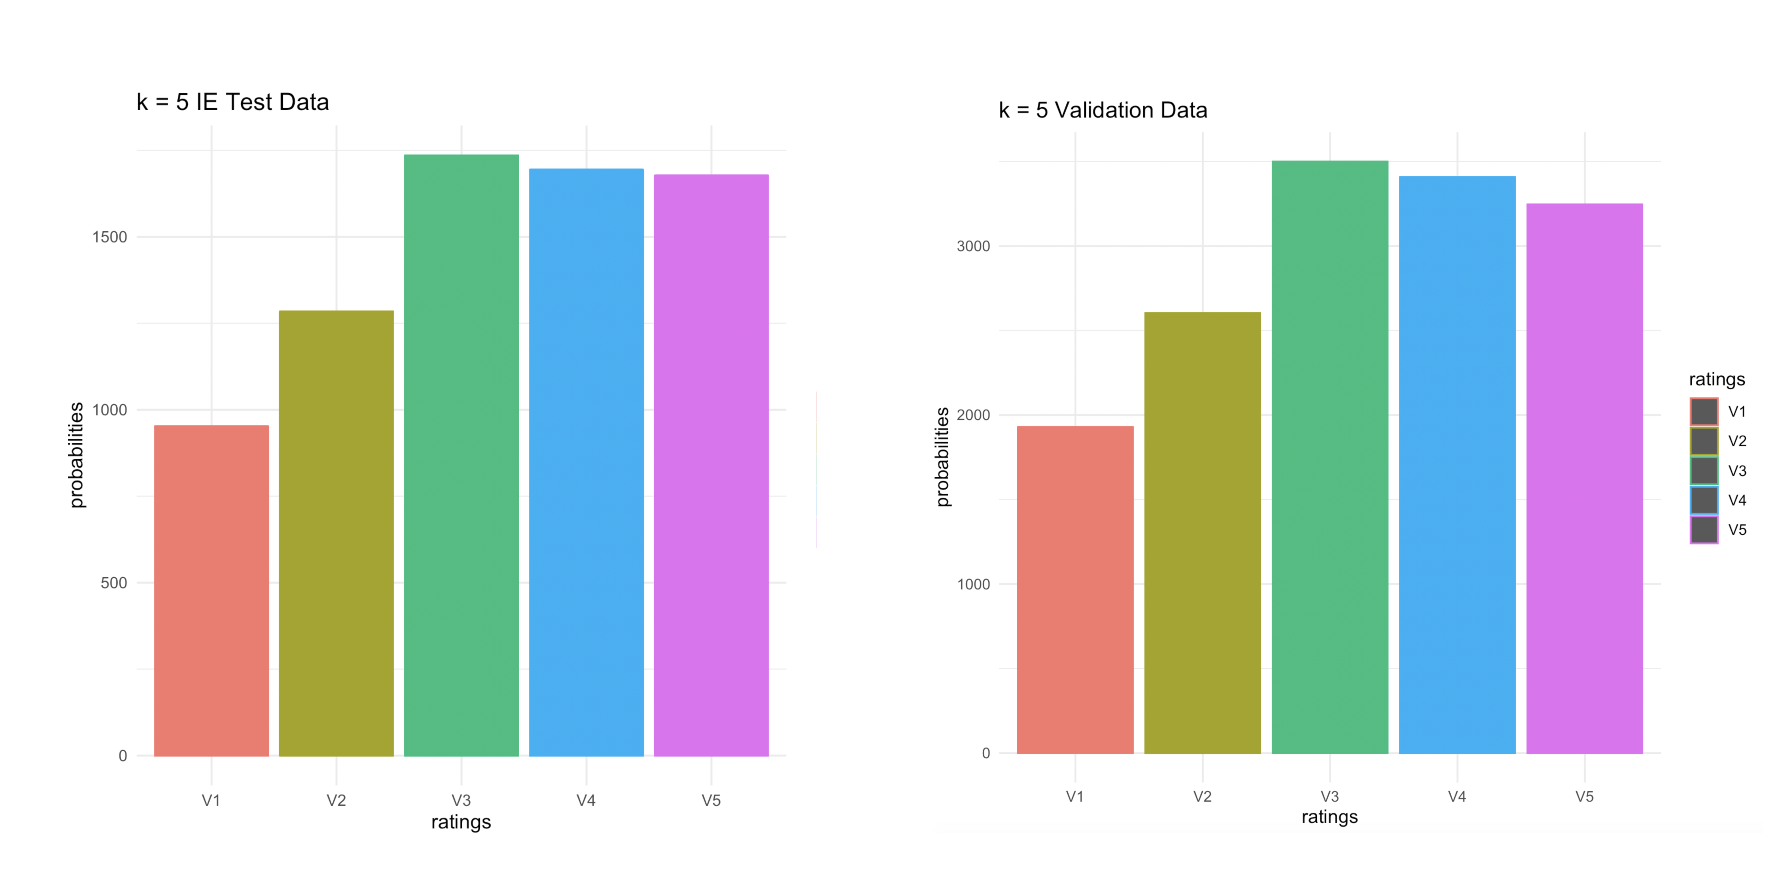
\includegraphics[scale=0.35]{k = 5 IE Bar Plot.png}
\caption{InstEval bar plots: k = 5}
\end{figure}

\begin{figure}[ht]
\centering
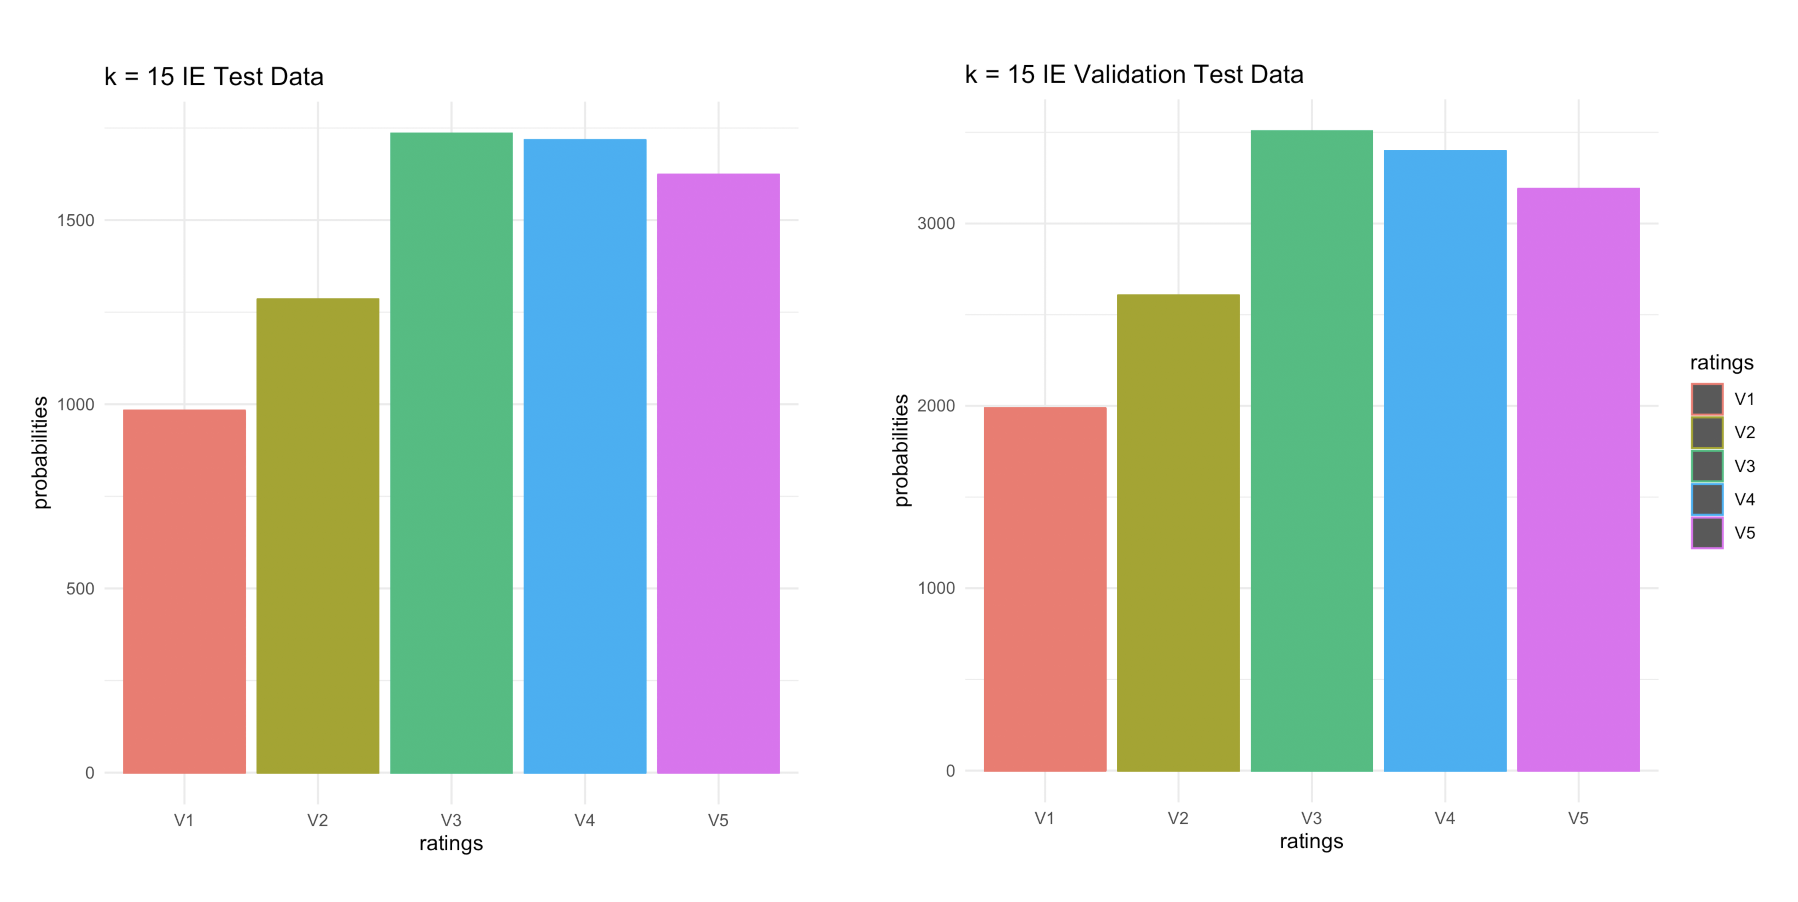
\includegraphics[scale=0.35]{k = 15 IE Bar Plot.png}
\caption{InstEval bar plots: k = 15}
\end{figure}

For both the k = 5 and k = 10 cases, we saw no noticable difference between the validation data bar plot and the test data bar plot. This signified that our validation data set and test data set were both properly sampled, resulting in a similar distribution of the ratings. We also saw no clear differences when comparing k = 5's bar plots to k = 15's bar plot, which may suggest that for InstEval, having k = 5 was good enough in representing the rating distribution. 

\begin{figure}[ht]
\centering
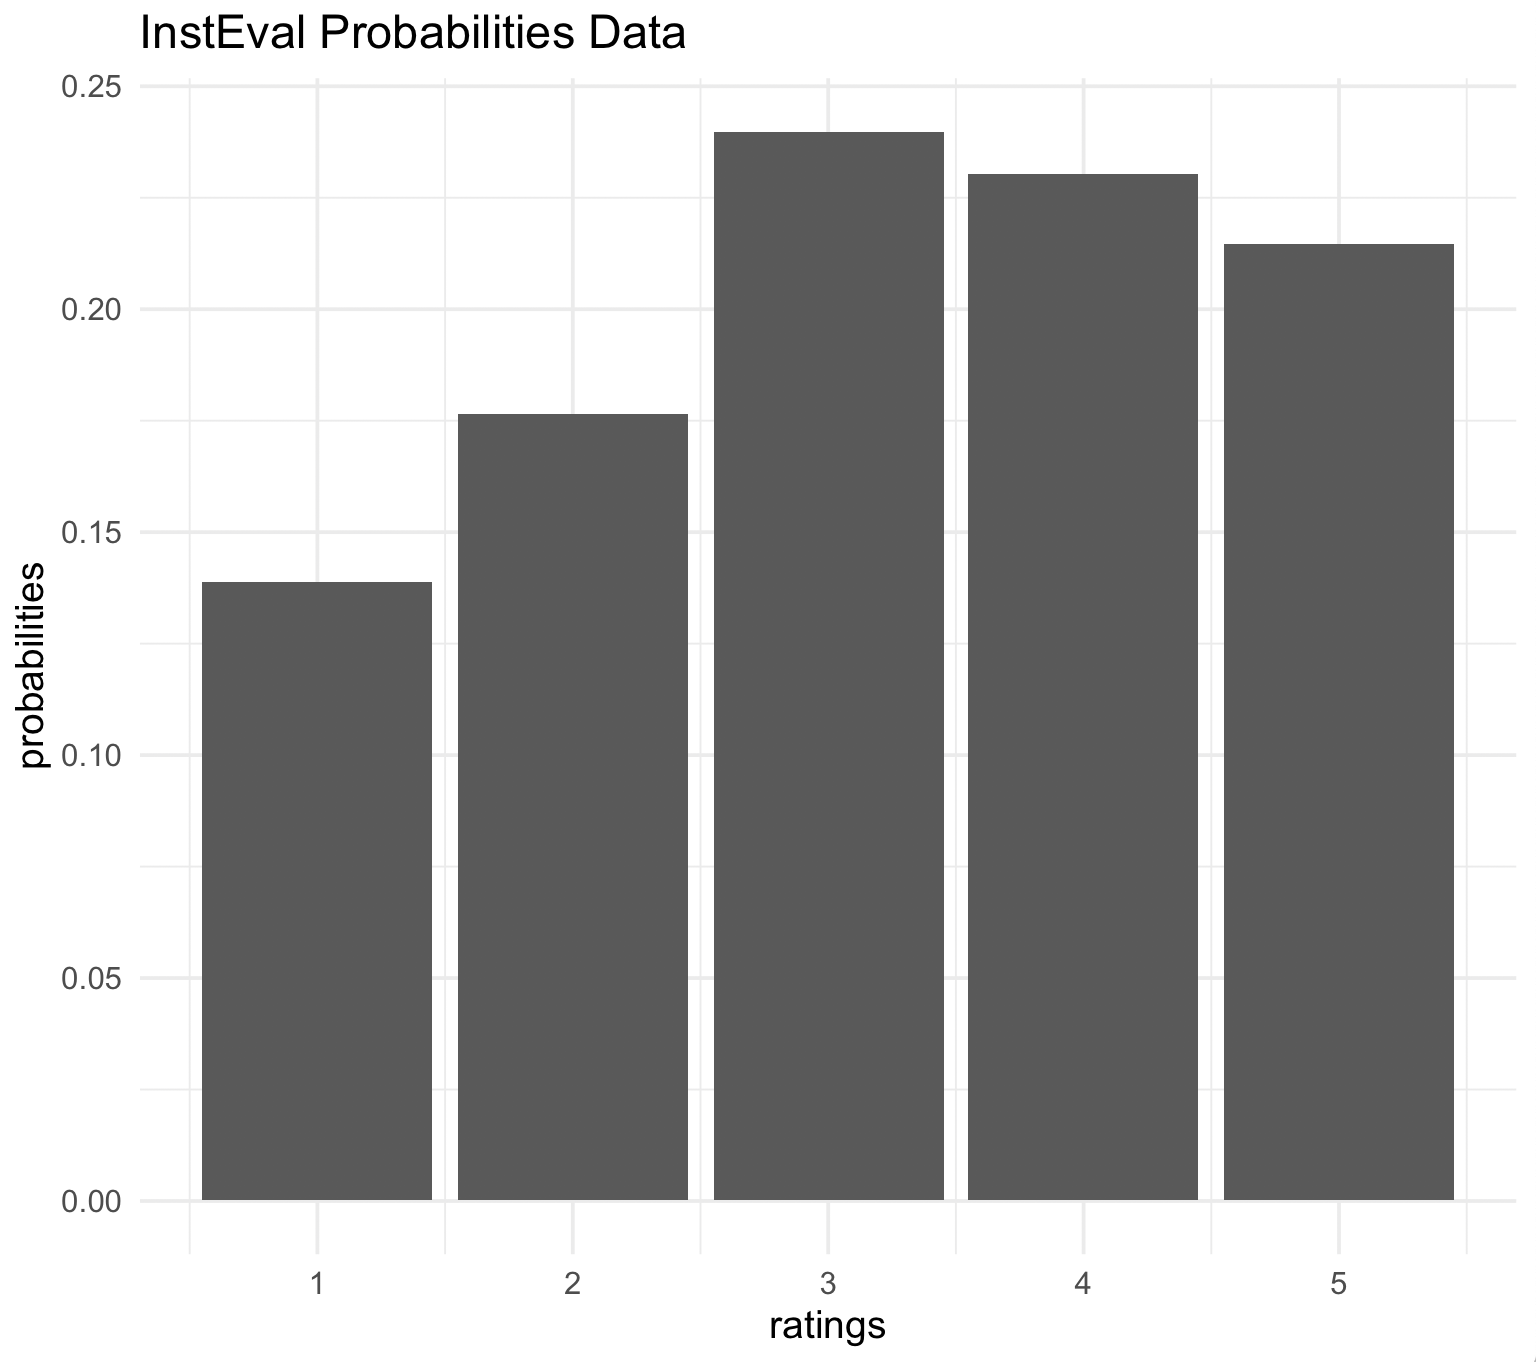
\includegraphics[scale=0.25]{IE Actual Probs.png}
\caption{InstEval actual rating distribution}
\end{figure}

Moreover, we can also see that those bar plots closely matched the bar plot for the actual ratings, which indicated that our kNN accurately matched the rating probability distribution of InstEval.

\begin{figure}[ht]
\centering
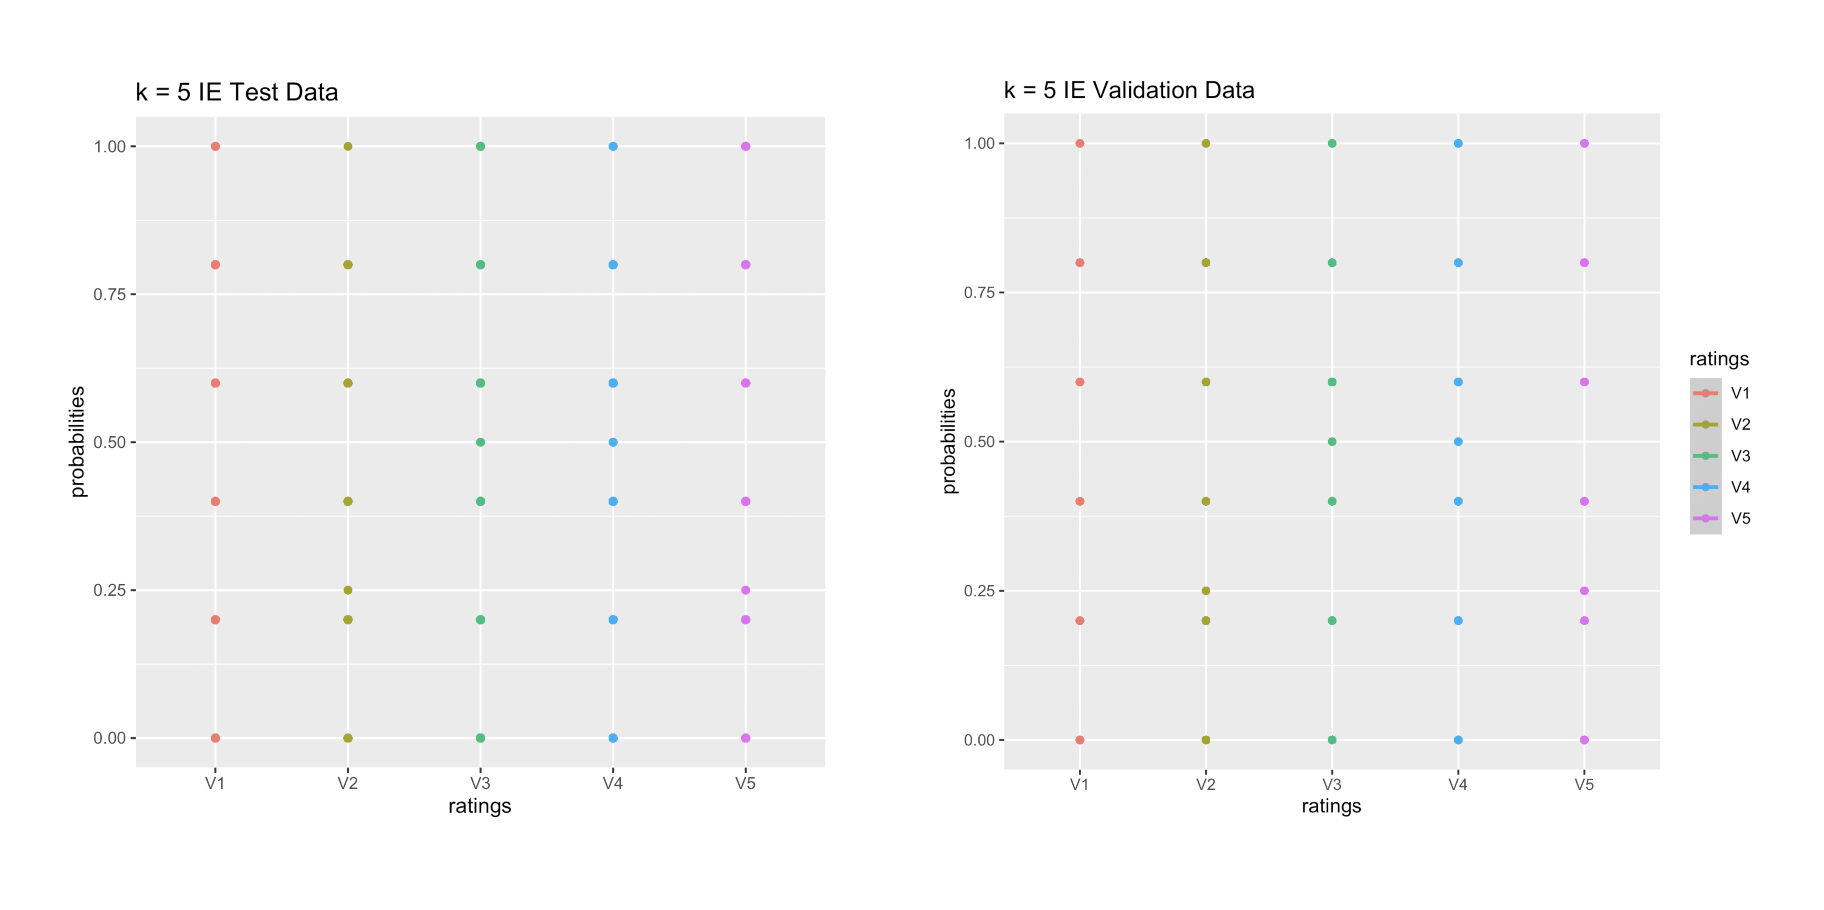
\includegraphics[scale=0.35]{k = 5 IE Scatter Plot.png}
\caption{InstEval scatter plots: k = 5}
\end{figure}

As for scatter plots, k = 5's scatter plots differed greatly to k = 15's ones. In the k = 5 case, the probabilities that a rating could have were roughly equally distributed; in the k = 15 case, the probabilities aggregated around the < 0.75 range. 

Nevertheless, such differences can be attributed to the value of k itself. Each rating's probability was calculated as the proportion of neighbours out of k nearest neighbours that had said rating. 

Therefore, for k = 5, the possible values for probability were {0.0,0.2,0.4,0.6,0.8,1.0}. The values 0.25 and 0.5 that were also in the plots indicated that some users that we had to predict only had 4 neighbours, since the possible probabilities for k = 4 were {0.0, 0.25, 0.5, 0.75, 1.0}. Here, we also note that while k = 4 has 5 possible probabilities, k = 5 has 6. Setting k to have a higher value thus allowing more possible probabilities, which explained why the scatter plots for k = 15 were more dense. 


\begin{figure}[ht]
\centering
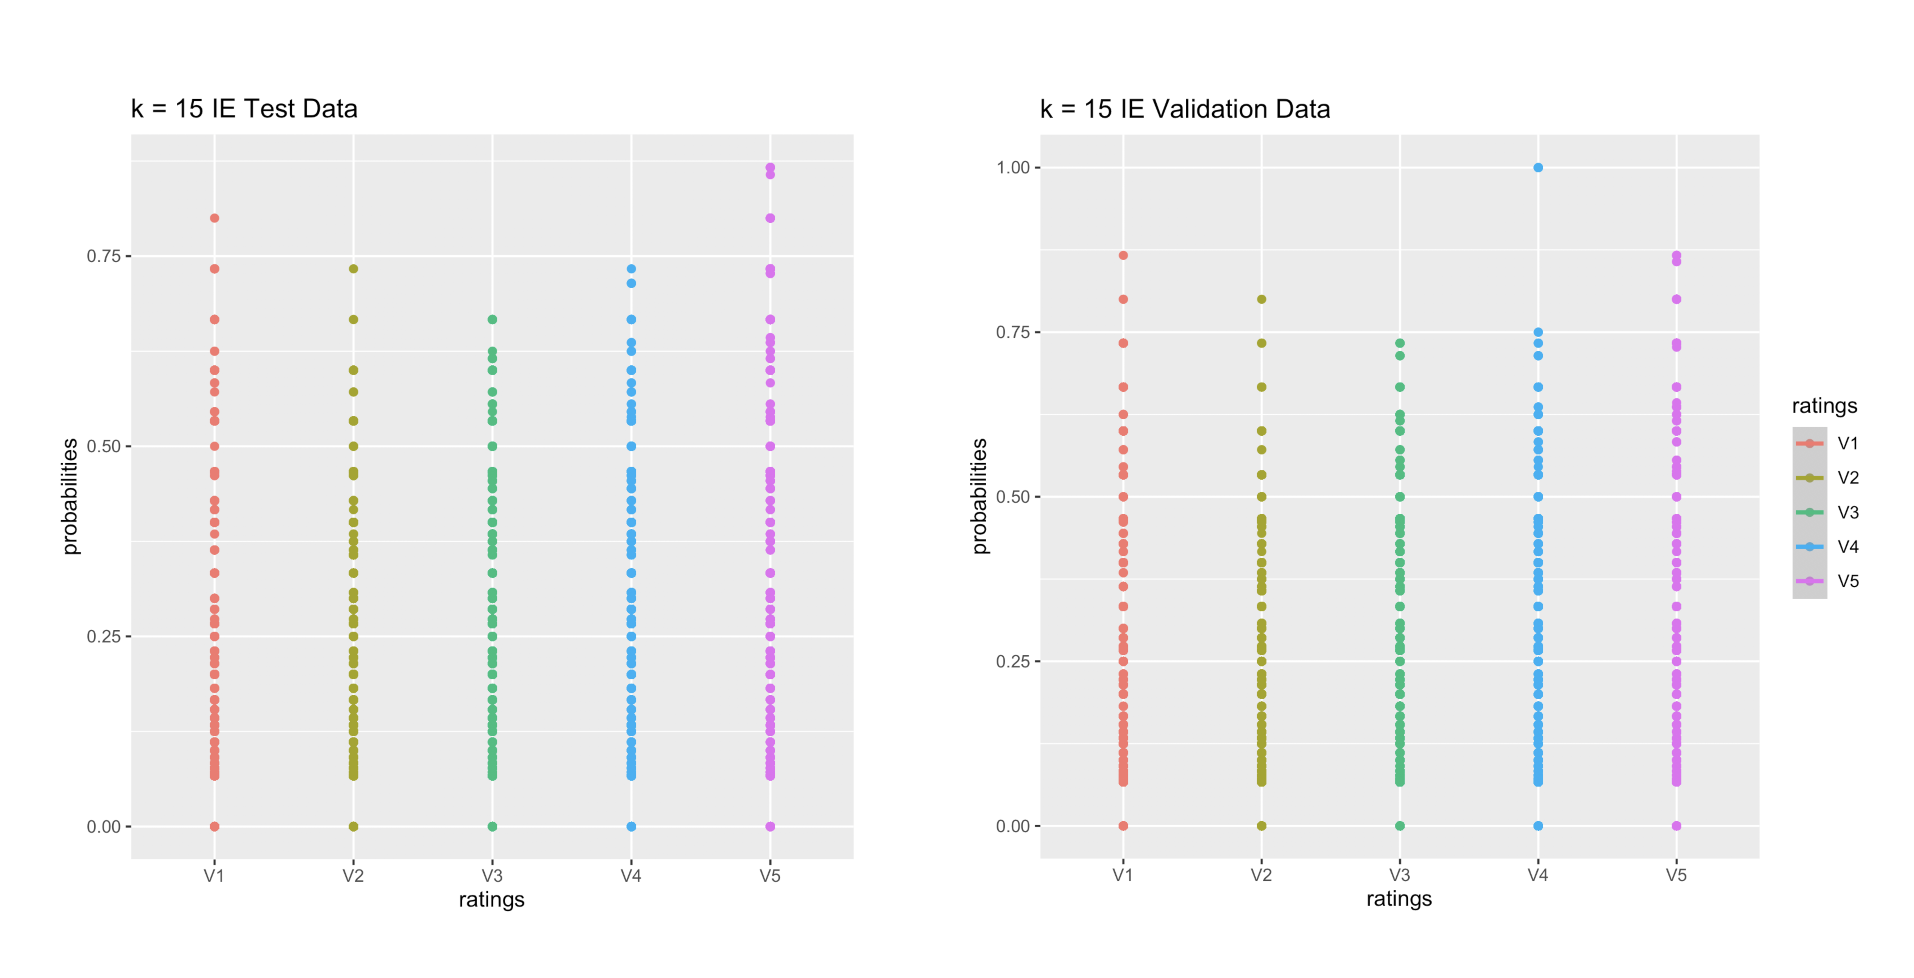
\includegraphics[scale=0.35]{k = 15 IE Scatter Plot.png}
\caption{InstEval scatter plots: k = 15}
\end{figure}

However, it was interesting to see that nearly all probabilities were less than 0.75, which indicated that kNN was rarely ever more than 75\% sure about a rating prediction (except for the rare case in rating 4 of the validation data).

\subsection{For SongList}

\begin{figure}[ht]
\centering
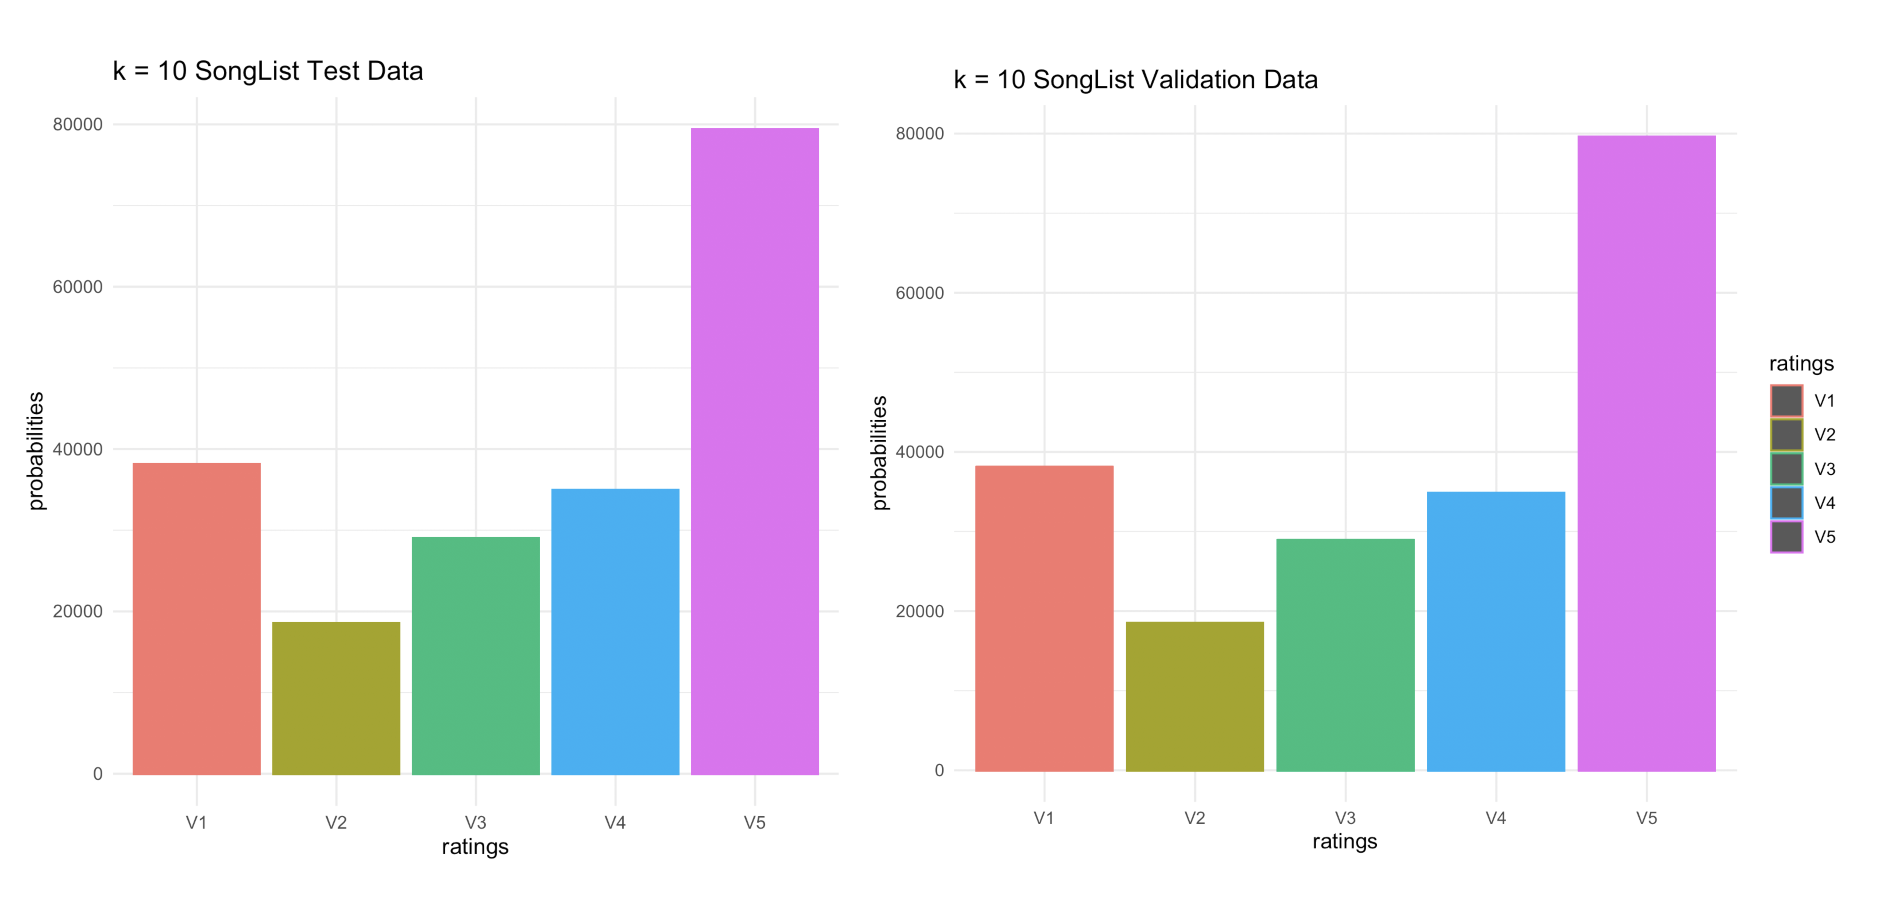
\includegraphics[scale=0.25]{k = 10 SL Bar Plot.png}
\caption{SongList Bar Plots: k = 5}
\end{figure}

Just like in InstEval, we see that the bar plots for the validation data and test data closely resembled each other, indicating that our data sets were properly sampled. Moreover, the bar plots were also similar to that of the actual rating, indicating that our kNN accurately matched the rating probability distribution of SongList as well.

\begin{figure}[ht]
\centering
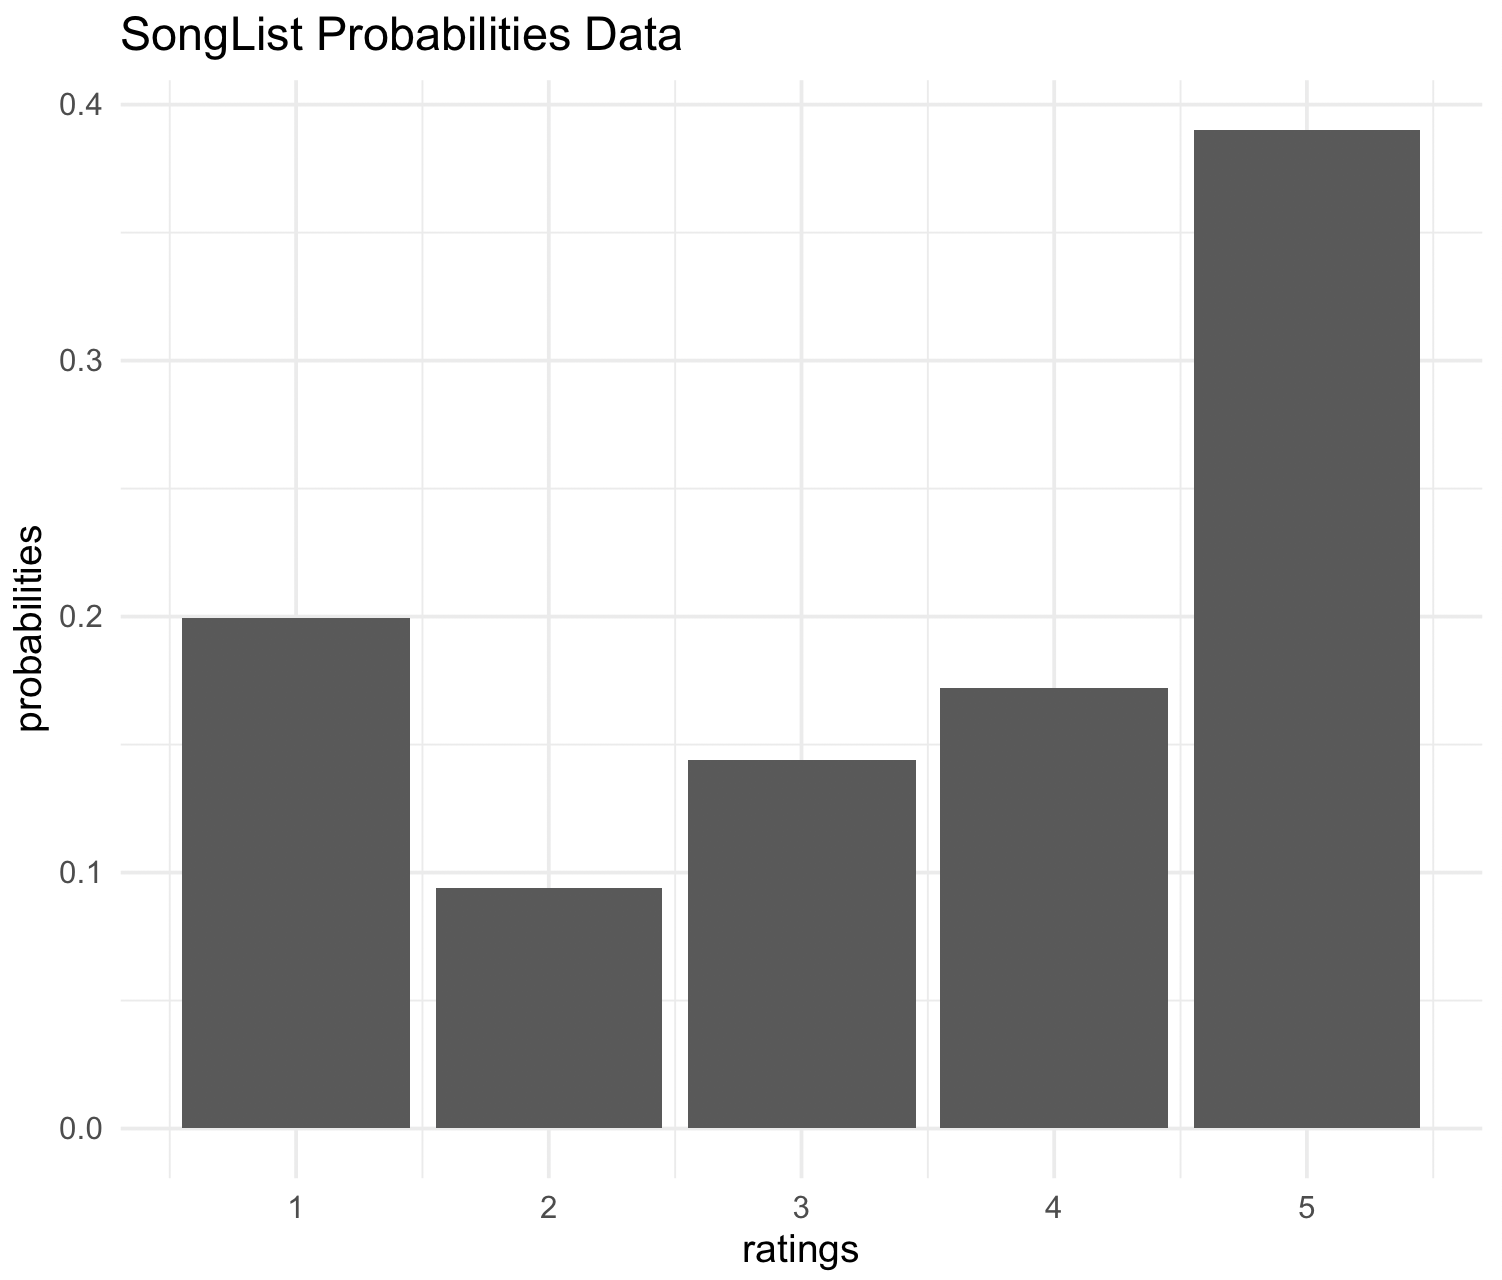
\includegraphics[scale=0.2]{SongList Actual Probs.png}
\caption{SongLIst Actual Rating Distribution}
\end{figure}

As for the scatter plots, the probabilities are slightly more distributed than the ones in InstEval's k = 15 case, and every rating had a 1.0 for some predictions. This could either be because the validation set and test set were larger, thereby increasing the chance of encountering a very obvious prediction case. Or it could be that since the training set was much larger, kNN had more data for its predictions and were generally more confident. 

\begin{figure}[ht]
\centering
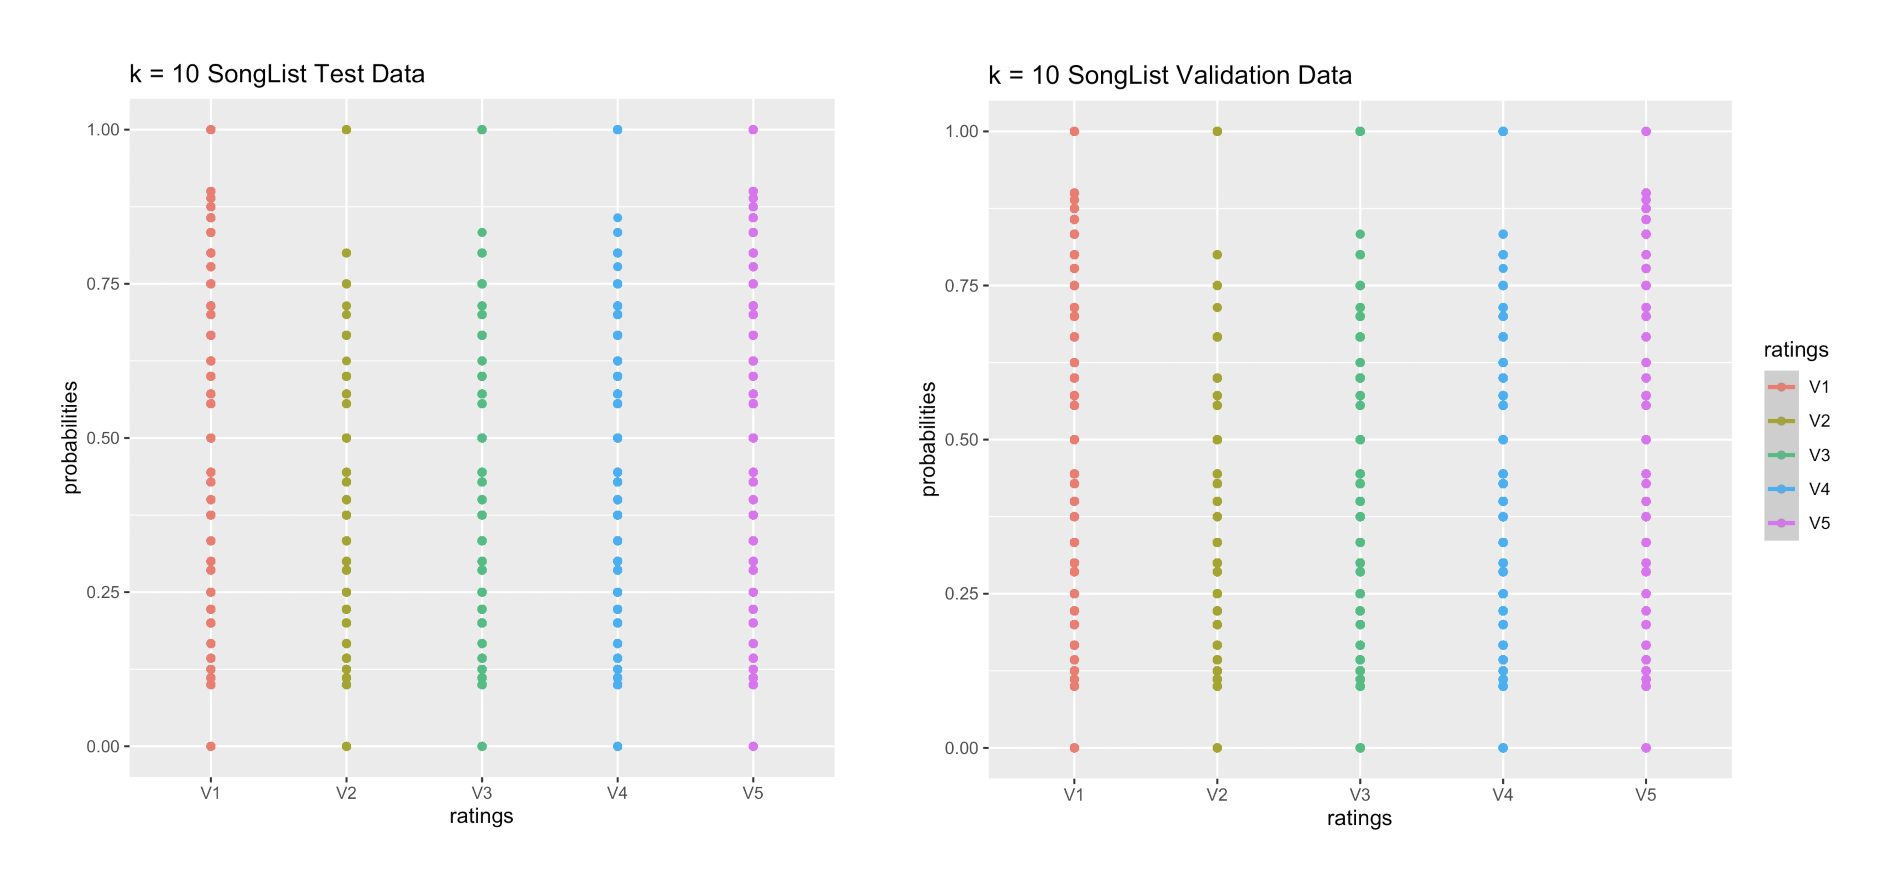
\includegraphics[scale=0.3]{k = 10 SL Scatter Plot.png}
\caption{SongList Scatter Plot}
\end{figure}

We believe the latter reasoning to be the case, as the validation and test accuracies for SongList were around 42\%, while said accuracies for InstEval were only around the 32-35\% range.

\section{CART - Classification and Regression Trees}
\subsection{Choosing a Strategy}
In order to add to our ratingProbsFit function the ability to predict the probability of each possible value of rating, we first considered two different strategies. The first was to replace the ratings with as many indicator variables as there were possible values for rating, as done in our implementation of the NMF case, run ctree for each of the indicator variables, and then have each outputted party object predict the probability of its corresponding rating, as determined by the indicator variable. The second strategy we considered, inspired by the random forests method, was to take some large number of samples from the inputted data set, run ctree on each sample, and for each row of a given test set, find the proportion of outputted party objects that predict a rating of 1, the proportion that predict a rating of 2, etc.

$\newline$
Later, we discovered that there was one more strategy we could consider, which was to call the party class's predict function with an additional argument: type="prob". Calling predict with type="prob" on a 1-row data frame named "newdata" produces an object of class "ecdf" that is also a function. If this object is assigned to a variable "ecdfFunc", it can then be called using "ecdfFunc(x)" where x is some numeric value. The value returned by this function call would then be the proportion of "similar" rows in the original training data that have ratings less than or equal to x, where "similar" rows are defined as the rows that are used to predict new cases that fall exactly in the terminal node which "newdata" would belong to. For example, if "newdata" corresponds to node 10, and node 10 in turn corresponds to a hundred rows of the original data, twenty of which have a rating less than or equal to 2, then "ecdfFunc(2)" would return 0.2. We plan to use the proportion computed by "ecdfFunc(x)" to estimate the probability that the rating is less than or equal to x.

$\newline$
The third strategy appeared to be no less accurate than our first two strategies in theory, and it also had the advantage of requiring less computation. Only a single tree would need to be generated in order to predict probabilities, while on the other hand the first strategy would require the generation of as many trees as there are possible values for rating, and the second strategy may require even more in order to accurately predict probabilities. Thus, we decided to use this last strategy to guide our implementation of the CART case.

\subsection{Using CART in ratingProbsFit}
When ratingProbsFit is run with the value of its argument predMethod equal to "CART", the return value of class recProbs contains the following information: the prediction method type ("CART"), the maximum possible rating, the mappings of user ID to mean user rating and item ID to mean item rating, and an object of class party obtained by running ctree with the data set passed in. Before running ctree, we must always transform the data first by replacing each user ID in the user ID column with the corresponding mean user rating and replacing each item ID in the item ID column with the corresponding mean item rating, for reasons described below in section 7.1. Calling ctree on the transformed data will form a recursive partitioning of the data space consisting of user mean and item mean rather than user ID and item ID. Thus, the mappings themselves are also saved in the return value, since any data we would like to predict ratings for must be transformed in the same manner before being passed to the party class's predict function.

\subsection{Predicting Rating Probabilities}
After transforming the data set "newXs", predict is called with the transformed data and the argument type set to "probs". The value returned by this call consists of a list, where each element is an empirical cumulative distribution function corresponding to one row of "newXs". The rating probabilities for each row of "newXs" can then be calculated using the following function:
\begin{lstlisting}
computeProbs <- function(ecdfFunc, maxRating) {
    probs <- sapply(1:maxRating, function(rating) 
        ecdfFunc(rating + 0.5) - ecdfFunc(rating - 0.5))
}
\end{lstlisting}
The above function "computeProbs" finds ecdf(1.5) to get the probability that the rating is a 1, ecdf(2.5) - ecdf(1.5) to get the probability that the rating is a 2 (i.e. between 1.5 and 2.5), etc.

\subsection{Results of Testing}
We tested our version of the CART prediction method for rating probabilities on the InstEval data set and the Song List data set, in each case partitioning the data set into a training set, a validation set, and a test set. For the InstEval data set, these account for 70\%, 20\%, and 10\% of the original data, respectively; for the Song List data set, they account for 80\%, 10\%, and 10\%, respectively. For each of the two data sets, we called ratingProbsFit with the training set and then called predict on the return value of the first function call with the validation set as the new data and later the test set as the new data. We then computed a comparison matrix for the validation set and one for the test set, the first column consisting of the average predicted probability that the rating is a 1, the average predicted probability that the rating is a 2, etc., and the second column corresponding to the actual proportion of ratings in the validation or test that are 1's, 2's, etc. The results for the Song List data set are below:

\begin{center}
    Validation Set
    \begin{tabular}{c|c|c}
        Rating & Avg predicted prob. & Actual proportion \\
        \hline
        1 & 0.19384487 & 0.195835 \\
        2 & 0.09295545 & 0.092725 \\
        3 & 0.14417024 & 0.143740 \\
        4 & 0.17298516 & 0.173775 \\
        5 & 0.39604427 & 0.393925 \\
    \end{tabular}
\end{center}

\begin{center}
    Test Set
    \begin{tabular}{c|c|c}
        Rating & Avg predicted prob. & Actual proportion \\
        \hline
        1 & 0.19436014 & 0.19655 \\
        2 & 0.09309556 & 0.09369 \\
        3 & 0.14442734 & 0.14330 \\
        4 & 0.17299311 & 0.17377 \\
        5 & 0.39512384 & 0.39269 \\
    \end{tabular}
\end{center}

$\newline$
In each case, the two columns are quite close - if we take each row in its percentage form, the two values are off by only a decimal point value. To get a measurement of the accuracy, we found the mean absolute prediction error (MAPE) for each comparison matrix, taking the first column to be our predicted values and the second column to be our actual values. The mean absolute prediction error turned out to be 0.001111986 for the validation data set and 0.001424474 for the test set, in each case less than a difference of 1\% in value (when the values in the matrix are expressed as percentages rather than decimal numbers).

$\newline$
We repeated the above process for the InstEval data set, computing the two comparison matrices, and found that the mean absolute prediction error was 0.002376233 for the validation data set and 0.004929582 for the test set, again in each less than a difference value of 1\% in value.


\section{Helper Functions}
\subsection{embedDataMeans}
In certain data sets, it would be difficult to perform predictions directly. There are data sets where the item IDs are not ordinal, hence they don't have underlying ordering. The solution is to create dummy variables for these IDs until moving forward to testing them one at a time. 
For example, say we're using CART as our prediction method and there is a possibility that there would be at most one data point that satisfied two conditions, this creates issues when making trees. Rather than using minsplit, we can embed the user ID and item ID to do dimension reduction. In this function, our goal was to create a new data frame, that includes the mapping between the userID and its mean ratings, as well as the itemID and its mean ratings. 

\subsection{dataToMatrix} 
The goal of this function is to make data handling for KNN and NMF easier. This functions turns our data frame into a data table, and creates a matrix like form of data with the userID's corresponding rating to itemID. With this function, the entries are replaced with NA if the user has not rated the item. 

\newpage
\section{Who Did What}
\subsection{Ynna}
I did the beginning phases and  handled the data. For example, I created a function to embed means. I also helped Leo create the probability predictions for lm.

$\newline$
In addition, I generated a function (along with Duong) to convert a data frame into a matrix to make data handling in NMF and kNN easier.  

$\newline$
Moreover, I wrote the general code to create the probability distribution visual aids. I then ran through all the data my group members generated from the predict function to create these charts and gathered important and significant observations that were used in the report.
 
\subsection{Jessica}
Jessica contributed to the CART portion of the project, including writing the CART-specific code of ratingProbsFit and predict.recProbs, testing our version of the CART prediction method, and measuring its accuracy, i.e. computing the "comparison matrices" and finding MAPEs.

\subsection{Duong}

Responsible for the experiment sets (training, validation, test) creation for both the InstEval and SongList datasets. In charge of the entirety of the kNN section.

\subsection{Leo}
I worked on the Logit component of this project. This includes the research, implementation, testing, and write up for the Logit method. 

$\newline$
In addition to this, I participated in the group discussions and helped discuss ideas for other implementations with the other group members. 

$\newline$
Moreover, I wrote the helper function that adds maxRatings extra columns to our data frame which converts the ratings into dummy variables.

\subsection{Tycho}
Completed NMF implementation and helped with ratingToDummy.


\newpage
\appendix
\section{TermProject.R}
For detailed comments, visit the repository
/ynnalecitona/ecs189g-termproject.

\begin{lstlisting}[language=R]
library(recosystem)
library(rectools)
library(partykit)
library(data.table)

ratingProbsFit <- function(dataIn,maxRating,predMethod,embedMeans,specialArgs){
  # Check for errors where using or not using embeded means with an incompatible method.
  # Will stop execution because of invalid inputs.
  if( embedMeans && predMethod == "NMF" ) {
    stop("Do not need to embed means for NMF.\n")
  }
  if( !embedMeans && predMethod == "CART" ) {
    stop("Mandatory for CART to embed means.\n")
  }
  dataInNoDummy <- dataIn
  dataIn <- ratingToDummy(dataIn, maxRating)

  if( predMethod == "logit" ) return(Logit(dataIn,maxRating))
  # Call the proper predition method.
  if( predMethod == "logit" && embedMeans ) {
    dataIn <- embedDataMeans(dataIn)
    return(Logit(dataIn,maxRating))
  }

  if( predMethod == "NMF" ) return(NMFTrain(dataIn,maxRating,specialArgs))

  if( predMethod == "kNN" ) return(KNN_setup(dataInNoDummy,maxRating,specialArgs))

  if( predMethod == "CART" ) return(CART(dataIn,maxRating,specialArgs))
}

predict <- function(probsFitOut,newXs) {
  if( probsFitOut$predMethod == "logit" ) return(LogitPredict(probsFitOut,newXs))
  if( probsFitOut$predMethod == "NMF" ) return(NMFPredict(probsFitOut,newXs))
  if( probsFitOut$predMethod == "kNN" ) return(KNN_predict(probsFitOut, newXs))
  if( probsFitOut$predMethod == "CART" ) return(CARTPredict(probsFitOut,newXs))
}

############################ LOGIT SECTION ############################

Logit <- function(dataIn, maxRating) {

  # Parameter Description
  # - dataIn: Data set with userID, itemID, Additional Predictors, Dummy Ratings
  # - maxRating: Maximum possible numerical rating that an item can be given

  # Verify that the dataIn dataframe is valid
  if(names(dataIn)[1] != "userID" | names(dataIn)[2] != "itemID") {
    write("logit: dataIn missing userID or itemID", stderr())
    return(status = -1)
  }

  # Declare the return object that will hold the linear models
  dataOut <- list(predMethod = "logit", maxRating = maxRating)

  # One vs. All approach to generate a binomial linear model for each possible rating
  for(i in 1:maxRating) {

    # Compute the index of the response variable
    index <- (ncol(dataIn) - maxRating + i)

    # Create the string for the formula
    responseName <- paste("r",toString(i), sep = "")
    form <- paste(responseName, "~ userID + itemID")

    # Create the logit model
    glmout <- glm(formula = form, data = dataIn, family = binomial, maxit = 50)

    # Add the glmout objects to the return object
    columnName <- paste("p",toString(i), sep = "")
    dataOut <- append(dataOut, list(glmout))
    names(dataOut)[2 + i] <- columnName
  }

  class(dataOut) <- "logit"

  return(dataOut)
}

LogitPredict <- function(probsFitOut, newXs) {

  # Generate the prediction probability for the first layer
  maxRatings <- probsFitOut[[2]]
  dataOut <- matrix(0, nrow = nrow(newXs), ncol = maxRatings)
  for(i in 1:maxRatings) {

    predictions <- predict.glm(probsFitOut[[2+i]], newXs, type = 'response')
    dataOut[,i] <- predictions
    colnames(dataOut)[i] <- paste("p",toString(i), sep = "")
  }

  return(dataOut)
}

############################ NMF SECTION ############################

NMFTrain <- function(dataIn,maxRating,specialArgs) {
	total_time <- Sys.time()
	# The list object to be outputted containing 3 values the prediction method and the list of trained models
	outProbFit <- vector('list', 3)
	names(outProbFit) <- c('predMethod', 'models', 'z')
	outProbFit$predMethod <- 'NMF'
	outProbFit$models <- vector('list', maxRating)
	givenRank <- FALSE

	# If the user does provide a rank then use that rank instead of tuning for a rank.
	if( 'rank' %in% names(specialArgs) ) {
		givenRank <- TRUE
	}

	# If the user wishes to increase the number of threads used to tune then they can be modified here.
	# The default is 1.
	nthread <- 1
	if ( 'nthread' %in% names(specialArgs) ) {
		nthread <- specialArgs$nthread
	}

	index1 <- specialArgs$index1

	# Over all the output columns
	for( i in 1:maxRating ) {
		# Factor in the user and item columns to get the current rating column
		nRatingCol <- i + 2
		
		reco <- Reco()

		# Init the training data for the current rating column
		training <- data_memory(dataIn[,1], dataIn[,2], dataIn[,nRatingCol], index1 = index1)
		if( givenRank ){
			reco$train(training, out_model = tempfile(), opt = list(dim = rank, nmf=TRUE, nthread = nthread))
		}
		else {
			print(paste("Begining to tune the Reco Model for Rating:", i))
			opts = list(dim = c(25,50,100,200,500,1000,2000), nmf = TRUE, costp_l1 = 0, costp_l2 = 0, costq_l1 = 0, costq_l2 = 0, lrate = 0.1, nmf = TRUE, nthread = nthread, progress = TRUE, verbose = TRUE)
			tuned <- reco$tune(training, opts = opts)

			fn <- paste(as.character(i),"SongYEs.data")
			saveRDS(tuned, file=fn)

			print(paste("Finished tuning the Reco Model for Rating:", i))
			reco$train(training, opts = tuned$min)
		}
			  	
		result <- reco$output(out_P = out_memory(), out_Q =  out_memory())
		outProbFit$models[[i]] <- result
	}

	return(outProbFit)
}

NMFPredict <- function(probsFitOut,newData) {
	nNewData <- nrow(newData)
	
	models <- probsFitOut$models
	nModels <- length(models)

	# Predictions with a column for each possible rating and a row for each new data input.
	preds <- matrix(nrow = nNewData, ncol = nModels)
	# For each new datum that we are given
	for(i in 1:nNewData) {
		# TODO remove print statement
		print(i)
		# For each model of a different rating
		for(j in 1:nModels) {
			newDatum <- newData[i,]
			# The prediction is equal to the dot product of the usersID row in P and the itemID col in Q 
			preds[i,j] <- models[[j]]$P[newDatum[[1]],] %*% models[[j]]$Q[newDatum[[2]],]
		}
		preds[i,] <- softmax(preds[i,])
	}
	# rows returned are the predictions of each rating for a new datum
	return(preds)
}

############################ KNN SECTION ############################

# specialArgs contains k (i.e. number of nearest neighbours)
KNN_setup <- function(dataIn, maxRating, specialArgs)
{
        trainData <- dataIn
        if ((.Machine$integer.max / length(unique(dataIn[,1]))) > length(unique(dataIn[,2]))) {
                dataSetSize <- "small"
        } else {
                dataSetSize <- "big"
        }
        maxRating <- maxRating
        KNNData <- list(trainData = dataIn, mode = dataSetSize, predMethod = "kNN",
                        k = specialArgs, maxRating = maxRating)
        class(KNNData) <- "recProbs"
        return(KNNData)
}

KNN_predict <- function(probsFitOut, newXs)
{
        if (probsFitOut$mode == "small")
                find_kNN_small(probsFitOut$trainData,
                               probsFitOut$k,
                               probsFitOut$maxRating,
                               newXs)
        else
                find_kNN_big(probsFitOut$trainData,
                             probsFitOut$k,
                             probsFitOut$maxRating,
                             newXs)
}

#-----------------------------kNN parameters checking-----------------------------

is_valid_values <- function(k, maxRating)
{
        valid <- TRUE
        if (k <= 0) {
                print("Error: k can't be less than or equal to 0.")
                valid <- FALSE
        }
        if (maxRating < 1) {
                print("Error: maxRating can't be less than 1.")
                valid <- FALSE
        }
        return(valid)
}

#-----------------------------kNN similarity funcs-----------------------------

# Similarity value: the bigger == the more similar

get_vlen <- function(v) sqrt(v %*% v)

#----------In-house similarity----------

inhouseSim <- function(potentialUser, targetUser)
{
        commItemsIdx <- !is.na(potentialUser) & !is.na(targetUser)
        if (sum(commItemsIdx) == 0) return(NaN)

        xvec <- potentialUser[commItemsIdx]
        yvec <- targetUser[commItemsIdx]
        yLen <- get_vlen(yvec)
        dotProd <- (xvec %*% yvec)
        pCos <- dotProd / yLen
        p_tCos <- ((xvec - yvec) %*% yvec) / yLen
        cosine <- dotProd / (get_vlen(xvec) * yLen)
        (pCos - p_tCos) * cosine
}

#-------------------------------kNN calculations-------------------------------

# Find users who have rated the target item.
find_rated_users <- function(dataIn, targetItemIdx)
{
        return(dataIn[which(!is.na(dataIn[,targetItemIdx])),])
}

# Calculate each rated user's similarity to the target user.
# Here is where to choose which similarity function to use.
# NOTE: Make sure to change the similarity function used in both the if and the else
#       statements if you're planning of using only one similarity function
calc_sims <- function(ratedUsers, targetUser, numRatedUsers)
{
        if (numRatedUsers == 1) {
                simVec <- inhouseSim(ratedUsers, targetUser)
        } else {
                simVec <- vector(mode = "numeric", length = nrow(ratedUsers))
                for (i in 1:numRatedUsers)
                        simVec[i] <- inhouseSim(ratedUsers[i,], targetUser)
        }
        return(simVec)
}

calc_rating_probs <- function(targetUser, targetItemIdx, ratedUsers,
                              simVec, k, maxRating)
{
        # Each element in simVec corresponds to the same element in ratedUsers
        sortOrder <- sort(simVec, decreasing = TRUE, na.last = TRUE, index.return = TRUE)
        if (length(sortOrder$ix) == 0) {
                # No nearest neighbours found
                # Return probability vector of all zeros.
                return(vector(mode = "numeric", length = maxRating))
        } else {
                if (length(sortOrder$ix) == 1) {
                        # Only 1 neighbor
                        nearestNeighbours <- ratedUsers
                        numNN <- 1
                        kNN <- nearestNeighbours[targetItemIdx]
                } else {
                        # If don't have k nearest neighbours,
                        #       use as many as there are
                        nearestNeighbours <- ratedUsers[sortOrder$ix,]
                        numNN <- min(k, nrow(nearestNeighbours))
                        kNN <- nearestNeighbours[1:numNN,targetItemIdx]
                }
                # Vector of each rating's frequency among k nearest neighbours
                ratings <- vector(mode = "numeric", length = maxRating)
                for (rating in 1:maxRating)
                        ratings[rating] = sum(kNN == rating) / numNN
                return(ratings)
        }
}

save_mat <- function(ratingPredMat, i, fileName)
{
        print("Saving matrix")
        name <- paste(fileName,".mat", i, sep="")
        write.csv(ratingPredMat, name, row.names = FALSE)
        # Only keep latest 5 iterations
        oldFileName <- paste(fileName,".mat", i - 5*10000, sep="")
        if (file.exists(oldFileName))
                unlink(oldFileName)
}

# find_kNN's assumptions:
#       1. newXs doesn't contain any new users or items
#       2. ratings have consecutive integer values, ranging from 1 to maxRating.

# This version of kNN is for cases where dataIn can be entirely converted into a matrix.
#       i.e. (# unique users * # unique items) < .Machine$integer.max
find_kNN_small <- function(dataIn, k, maxRating, newXs,
                           fileName = NULL, verbose = FALSE, progressSaving = FALSE)
{
        if(is_valid_values(k, maxRating) == FALSE)
                return(-1)

        dataMat <- dataToMatrix(dataIn)
        ratingPredMat <- matrix(nrow = nrow(newXs), ncol = maxRating)
        for (i in 1:nrow(newXs)) {
                if (verbose)
                        print(i)
                targetUserIdx <- which(rownames(dataMat) == newXs[i,1])
                targetItemIdx <- which(colnames(dataMat) == newXs[i,2])

                if (!is.na(dataMat[targetUserIdx, targetItemIdx])) {
                        # Known rating
                        ratings <- vector(mode = "integer", length = maxRating)
                        ratings[dataMat[targetUserIdx, targetItemIdx]] = 1
                        ratingPredMat[i,] <- ratings
                } else {
                        ratedUsers <- find_rated_users(dataMat, targetItemIdx)
                        targetUser <- dataMat[targetUserIdx,]
                        numRatedUsers <- sum(!is.na(dataMat[,targetItemIdx]))
                        simVec <- calc_sims(ratedUsers, targetUser, numRatedUsers)
                        ratingPredMat[i,] <- calc_rating_probs(targetUser, targetItemIdx, ratedUsers, simVec, k, maxRating)
                }
                if (progressSaving && i %% 10000 == 0)
                        save_mat(ratingPredMat, i, fileName)
        }
        return(ratingPredMat)
}

find_kNN_big <- function(dataIn, k, maxRating, newXs,
                         fileName = NULL, verbose = FALSE, progressSaving = FALSE)
{
        if(is_valid_values(k, maxRating) == FALSE)
                return(-1)
        # byrow = TRUE allows us to replace a matrix's row with a vector
        ratingPredMat <- matrix(nrow = nrow(newXs), ncol = maxRating, byrow = TRUE)
        for (i in 1:nrow(newXs)) {
                if (verbose)
                        print(i)
                foundRating <- dataIn[,1] == newXs[i,1] & dataIn[,2] == newXs[i,2]

                # Assume no repeated rating
                if (sum(foundRating) > 0) {
                        # Known rating
                        ratings <- vector(mode = "integer", length = maxRating)
                        ratings[dataIn[foundRating,3]] = 1
                        ratingPredMat[i,] <- ratings
                } else {
                        # Get users who have rated item newXs[i,2]
                        ratedUsersIDs <- dataIn[which(dataIn[,2] == newXs[i,2]),1]
                        targetUserID <- newXs[i,1]

                        ratedUsersIdx <- which(dataIn[,1] %in% ratedUsersIDs)
                        targetUserIdx <- which(dataIn[,1] %in% targetUserID)

                        dataExtract <- dataToMatrix(dataIn[c(ratedUsersIdx,targetUserIdx),])

                        targetUserIdx <- which(rownames(dataExtract) == newXs[i,1])
                        targetItemIdx <- which(colnames(dataExtract) == newXs[i,2])

                        ratedUsers <- dataExtract[-targetUserIdx,]
                        targetUser <- dataExtract[targetUserIdx,]
                        numRatedUsers <- length(ratedUsersIDs)
                        simVec <- calc_sims(ratedUsers, targetUser, numRatedUsers)
                        ratingPredMat[i,] <- calc_rating_probs(targetUser, targetItemIdx,ratedUsers, simVec, k, maxRating)
                }
                if (progressSaving && i %% 10000 == 0)
                        save_mat(ratingPredMat, i, fileName)
        }
        return(ratingPredMat)
}

############################ CART SECTION ############################

CART <- function(dataIn,maxRating,specialArgs) {
  recProbs <- list(predMethod="CART", maxRating=maxRating)
  class(recProbs) <- "recProbs"

  # map user ID to user's mean rating, item ID to item's mean rating
  mappings <- embedDataMeans(dataIn)
  recProbs$mappings <- mappings
  dataIn$userID <- mappings$user_mean
  dataIn$itemID <- mappings$item_mean

  args <- specialArgs
  args$formula <- as.formula('rating ~ .')
  args$data <- dataIn

  ctout <- do.call(ctree, args)
  recProbs$party <- ctout
  recProbs
}

CARTPredict <- function(probsFitOut,newXs) {
  # transform newXs
  lookUp <- function(onekey, keys, vals) vals[which(as.character(keys) == as.character(onekey))[1]]
  newXs$userID <- sapply(newXs$userID, lookUp, probsFitOut$mappings$userID, probsFitOut$mappings$user_mean)
  newXs$itemID <- sapply(newXs$itemID, lookUp, probsFitOut$mappings$itemID, probsFitOut$mappings$item_mean)

  ratings <- predict(probsFitOut$party, newXs, type="prob")

  computeProbs <- function(ecdfFunc, maxRating) probs <- sapply(1:maxRating, function(rating) ecdfFunc(rating + 0.5) - ecdfFunc(rating - 0.5))
  ratingProbs <- sapply(ratings, computeProbs, probsFitOut$maxRating)
  t(ratingProbs)
}

############################ HELPER FUNCTIONS ############################
embedDataMeans <- function(dataIn) {
  # mean ratings for a user
  ud <- formUserData(dataIn)
  mean_users <- sapply(ud, function(oneusr) mean(oneusr$ratings))

  # mean ratings for an item
  # switch userid and itemid so that
  udReversed <- formUserData(dataIn[,c('itemID', 'userID', 'rating')])
  mean_items <- sapply(udReversed, function(oneitm) mean(oneitm$ratings))

  # create new columns that holds the user_mean and item_mean
  # assuming that the user named the column headings as userID and itemID
  dataIn$user_mean <- mean_users[dataIn$userID]
  dataIn$item_mean <- mean_items[dataIn$itemID]

  # return a data frame that maps userid with user mean and
  # itemid with item mean
  mappings <- as.data.frame(dataIn[, c('userID', 'user_mean', 'itemID', 'item_mean')])
  return(mappings)
}

dataToMatrix <- function(dataIn) {
  # turns data frame into data.table which is more enhanced than data.frame
  dt <- as.data.table(dataIn)

  # creates the table entries, and fill empty ones with NAs
  userID <- names(dataIn)[1]
  itemID <- names(dataIn)[2]
  valueName <- names(dataIn)[3]
  formula <- paste(c(userID, itemID), collapse = '~')
  table <- dcast(dt, formula, fill = NA, value.var=valueName)

  # The first column of table will be the userID, which we don't need in our matrix
  mat <- as.matrix(table[,-1])

  # Assign the row names of the new matrix with our userIDs
  rNames <- as.list(table[,1])
  rNames <- rNames[[names(rNames)]]
  row.names(mat) <- rNames
  return(mat)
}

ratingToDummy <- function(data, maxRatings) {

  # Verify that maxRating is valid
  if(!(maxRatings > 0)) {
    write("ratingToDummy: maxRating is an invalid number", stderr())
    return(status = -1)
  }

  # Extract the ratings from the data
  ratings <- data[,3]
  data <- data[,-3]

  # Add the dummy variable ratings to the end of the data
  for(i in 1:maxRatings) {

    # Create the name for the new column in the format "r + rating number"
    name <- paste("r", toString(i), sep = "")

    # Each value in the column represents a bool that is true if the user gave
    # the item the rating "i"
    data[,(ncol(data) + 1)] <- as.integer(ratings == i)

    # Add the name to newly created column
    names(data)[ncol(data)] <- name
  }

  return(data)
}

softmax <- function(values, z = 1) {
  temp <- values * z
  expValues <- sapply(temp, exp)
  return( expValues/sum(expValues) )
}
\end{lstlisting}

\newpage
\section{Probability Distributions Scatter Plot Generator}
For detailed comments, visit the repository
/ynnalecitona/ecs189g-termproject.
\begin{lstlisting}[language=R]
library(ggplot2)
library(reshape)
generate_scatter_plot <- function(data_to_plot) {
    data_to_plot[] <- lapply(data_to_plot, unlist)
    data_to_plot <- melt(data_to_plot)
    names(data_to_plot) <- c("ratings", "probabilities")
    scatter_plot <- ggplot(data_to_plot, 
    aes(ratings, probabilities, 
    col= ratings)) + geom_point() + stat_smooth()
    scatter_plot
    
    
}
\end{lstlisting}

Example Output:
\begin{figure}[ht]
\centering
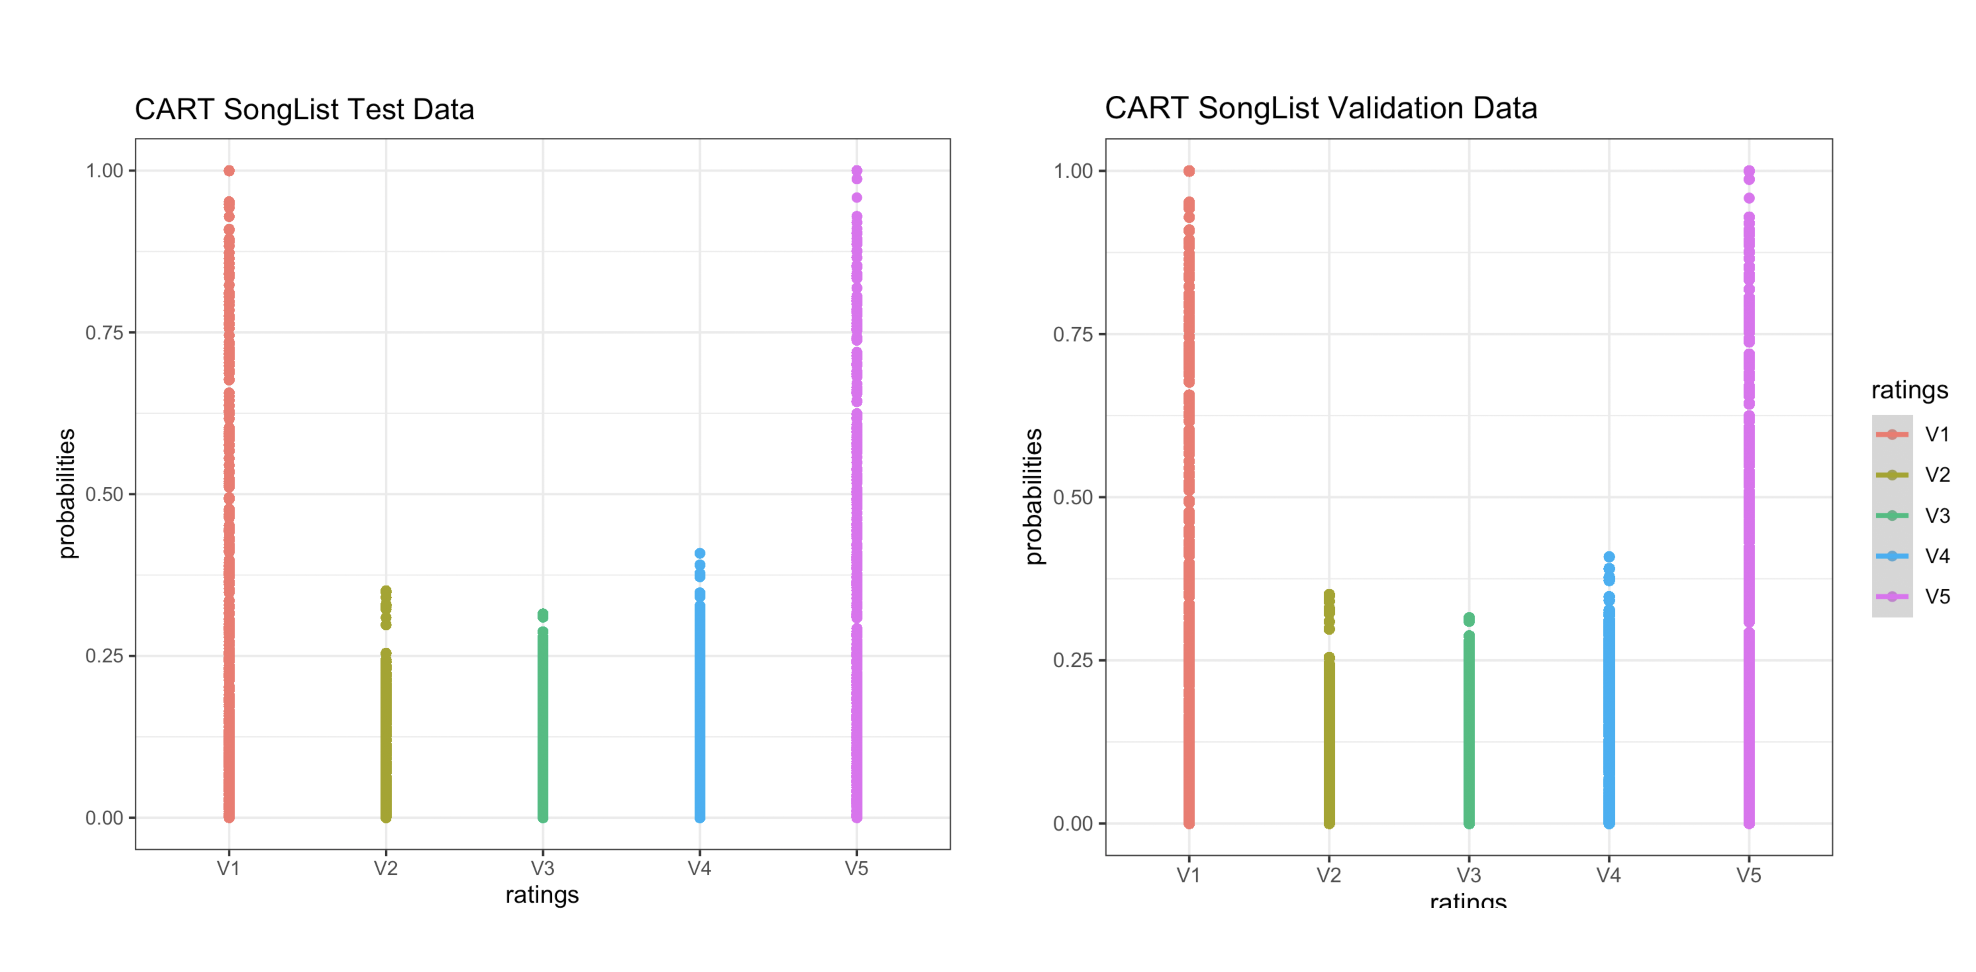
\includegraphics[scale=0.3]{CART SongList Scatter Plot.png}
\caption{CART SongList Scatter Plot}
\label{fig:universe}
\end{figure}


\section{Probability Distributions Bar Plot Generator}
\begin{lstlisting}[language = R]
library(ggplot2)
library(reshape)
generate_bar_plot <- function(data_to_plot) {
  data_to_plot[] <- lapply(data_to_plot, unlist)
  data_to_plot <- melt(data_to_plot)
  names(data_to_plot) <- c("ratings", "probabilities")
  bar_plot <- ggplot(data_to_plot, 
  aes(ratings, probabilities, col= ratings)) + 
  geom_bar(stat="identity") + theme_minimal()
  bar_plot
}
\end{lstlisting}

Example Output:
\begin{figure}[ht]
\centering
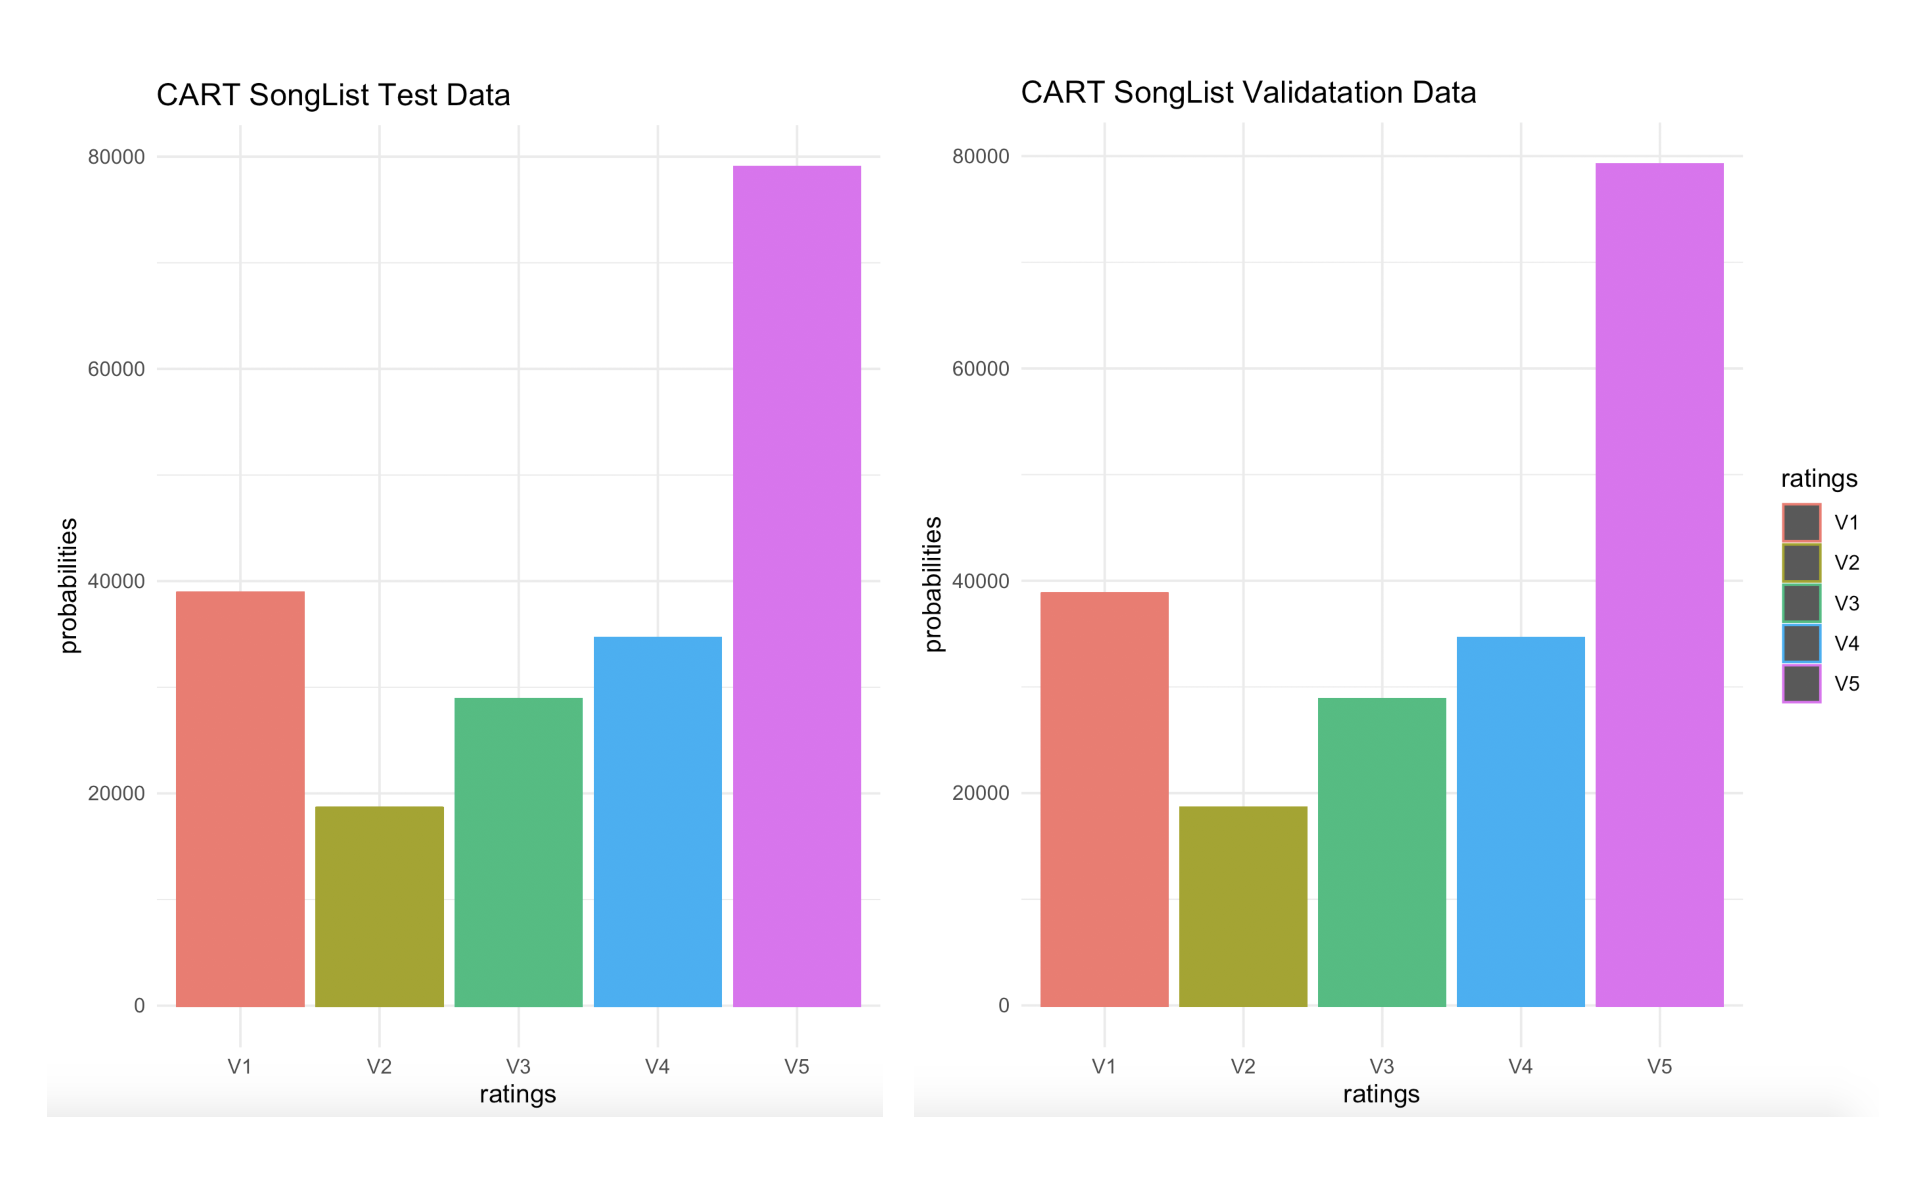
\includegraphics[scale=0.3]{CART SongList Bar Plot.png}
\caption{CART SongList Bar Plot}
\label{fig:universe}
\end{figure}


\section {Experiment Sets Generator}
For detailed comments, visit the repository
/ynnalecitona/ecs189g-termproject.
\begin{lstlisting}[language = R]
does_contain_all <- function(targetList, checkList)
{
    numElementsLacked <- sum(!(checkList %in% targetList))
    return(numElementsLacked == 0)
}
sampling_data <- function(dataIn, sampleSize, 
verbose = FALSE) 
{
    if (sampleSize > nrow(dataIn)) {
        print("Error: Sample size greater than data size")
        return(-1)
    }
    uniqueUsersTotal <- unique(dataIn[,1])
    uniqueItemsTotal <- unique(dataIn[,2])
    samplingIdx <- sample(1:nrow(dataIn), sampleSize)
    sampleData <- dataIn[samplingIdx,]
    i <- 1
    while (!does_contain_all(sampleData[,1], 
    uniqueUsersTotal) || !does_contain_all(sampleData[,2], 
    uniqueItemsTotal)) {
        samplingIdx <- sample(1:nrow(dataIn), sampleSize)
        sampleData <- dataIn[samplingIdx,]
        i <- i + 1
    }
    if (verbose) {
        print("Trials needed: ")
        print(i)
    }
    return(sampleData)
}

create_experiment_sets <- function(dataIn, ratio)
{
    if (sum(ratio) != 1) {
        print("Invalid ratios")
        return(-1)
    }

    trainSetSize <- floor(nrow(dataIn) * ratio[1])
    validationSetSize <- floor(nrow(dataIn) * ratio[2])
    testSetSize <- nrow(dataIn) - trainSetSize 
    - validationSetSize

    trainSet <- sampling_data(dataIn, trainSetSize)
    print("Train set sampling done")

    sampledRows <- as.numeric(rownames(trainSet))
    leftovers <- dataIn[-sampledRows,]
    rownames(leftovers) <- 1:nrow(leftovers)

    samplingIdx <- sample(1:nrow(leftovers), 
    validationSetSize)
    validationSet <- leftovers[samplingIdx,]
    print("Validation set sampling done")

    sampledRows <- as.numeric(rownames(validationSet))
    testSet <- leftovers[-sampledRows,]
    print("Test set sampling done")

    experiment_sets <- list(trainSet = trainSet, 
    validationSet = validationSet, testSet = testSet)
    class(experiment_sets) <- "expSets"
    return(experiment_sets)
}

save_experiment_sets <- function(expSets)
{
    trainSet <- expSets$trainSet
    validationSet <- expSets$validationSet
    testSet <- expSets$testSet
    write.csv(trainSet, "train.data", row.names = FALSE)
    write.csv(validationSet, "validation.data", 
    row.names = FALSE)
    write.csv(testSet, "test.data", row.names = FALSE)
}

\end{lstlisting}

\section{Generate Partitions}
\begin{lstlisting}[language=R]
  test <- setdiff(1:nrow(dataIn), train)

  n <- floor(0.95 * nrow(dataIn))
  cond <- FALSE
  
  while(!cond) {

    trainIndx <- sample(nrow(dataIn), n)
    testIndx <- setdiff(1:nrow(dataIn), trainIndx)
    cond <- TRUE

    for(factor in names(dataIn)[1:2]) {
      trainLevels <- dataIn[trainIndx, factor]
      testLevels <- dataIn[testIndx, factor]
      
      if(!all(testLevels %in% trainLevels)) {
        cond <- FALSE
      }
    }
  }
\end{lstlisting}

\section{Aesthetic R Code in Latex}
\raggedright\url{https://tex.stackexchange.com/questions/374001/insert-r-code-in-latex}

\section{Cross Validation with Factors}
\raggedright\url{https://stackoverflow.com/questions/19946930/r-cross-validation-on-a-dataset-with-factors}

\section{Potential Similarity Functions Used in kNN}
\label{sec:kNNSim}

1. l-p norm (Manhattan, Euclidean, Chebychev): 

$\newline$
\raggedright\url{https://dataaspirant.com/2015/04/11/five-most-popular-similarity-measures-implementation-in-python/}

$\newline$
2. Jaccard similarity:

$\newline$
\raggedright\url{https://dataaspirant.com/2015/04/11/five-most-popular-similarity-measures-implementation-in-python/}

$\newline$
\raggedright\url{https://en.wikipedia.org/wiki/Jaccard_index#Tanimoto_Similarity_and_Distance}

$\newline$
3. Radial basis function kernel:

$\newline$
\raggedright\url{https://en.wikipedia.org/wiki/Radial_basis_function_kernel}

$\newline$
4. Cosine similarity:

$\newline$
\raggedright\url{https://en.wikipedia.org/wiki/Cosine_similarity}

$\newline$
5. Dot product:

$\newline$
\raggedright\url{https://developers.google.com/machine-learning/clustering/similarity/measuring-similarity}

$\newline$
6. Correlation:

$\newline$
\raggedright\url{http://www.analytictech.com/mb876/handouts/distance_and_correlation.htm}

\end{document}

